\documentclass{beamer}
%
% Choose how your presentation looks.
%
% For more themes, color themes and font themes, see:
% http://deic.uab.es/~iblanes/beamer_gallery/index_by_theme.html
%
\mode<presentation>
{
  \usetheme{Madrid}      % or try Darmstadt, Madrid, Warsaw, ...
  \usecolortheme{seahorse} % or try albatross, beaver, crane, ...
  \usefonttheme{serif}  % or try serif, structurebold, ...
  \setbeamertemplate{navigation symbols}{}
  \setbeamertemplate{caption}[numbered]
} 


\usepackage[english]{babel}
\usepackage{kotex}
%\usepackage[utf8x]{inputenc}

\title[게임수학 강의]{ 게임 수학 강의 노트 part 1}
\author{강영민}
\institute{동명대학교}
\date{2015년 2학기}

\begin{document}

%%%%%%%%%%%%%%%%%%%%%%%%%%%%%%%%%%%%%%%%%%%%%%%%%%%%%%%%%
\begin{frame}
  \titlepage
\end{frame}

% Uncomment these lines for an automatically generated outline.
%\begin{frame}{Outline}
%  \tableofcontents
%\end{frame}


%%%%%%%%%%%%%%%%%%%%%%%%%%%%%%%%%%%%%%%%%%%%%%%%%%%%%%%%%
\begin{frame}{벡터란 무엇인가?}
\begin{itemize}
\item 벡터의 의미
  \begin{itemize}
  \item 벡터(vector)는 ‘나르다’라는 의미의 라틴어 동사 ‘vehere'에서 유래
  \item ‘무엇인가를 나르는 것’이라는 의미
  \item 벡터라는 것은 무엇인가를 옮겨 놓는 역할을 수행한다.
  \end{itemize}
\end{itemize}

\begin{itemize}
\item 수학과 물리학에서의 개념
  \begin{itemize}
  \item 크기와 방향으로 결정되는 양(量, quantity)
  \item 방향량(方向量)이라고도  함.
  \item 예: 힘(force)은 크기만으로는 그 성질을 온전히 표현할 수 없고, 방향도 같이 고려해야 하므로 벡터로 표현된다.
  \end{itemize}
\end{itemize}

\begin{block}{벡터}
수학자들은 자연 현상의 많은 것들이 수로 표현될 수 있음을 알았는데, 하나의 숫자로 충분히 표현할 수 있지만 하나 이상의 수가 필요한 경우도 있다. 
이러한 양을 벡터(vector)라고 부른다.
\end{block}

\end{frame}

%%%%%%%%%%%%%%%%%%%%%%%%%%%%%%%%%%%%%%%%%%%%%%%%%%%%%%%%%


%%%%%%%%%%%%%%%%%%%%%%%%%%%%%%%%%%%%%%%%%%%%%%%%%%%%%%%%%
\begin{frame}{벡터의 개념}

\begin{itemize}
\item 물리적 현상 등을 표현할 때 - 대상을 양(量, quantity)으로 표현 
\item 이 양은 스칼라(scalar) 혹은 벡터(vector)
	\begin{itemize}
	\item 스칼라 값은 오로지 크기만으로 완전히 그 양을 표현할 수 것으로서 물체의 질량, 소요된 시간, 길이, 열량 등이 해당
	\item 벡터(vector)는 이와 달리 크기와 함께 방향도 같이 존재하는 양으로 힘, 속도, 변위와 같은 양이 바로 여기에 해당
	\end{itemize}
\end{itemize}

\begin{itemize}
\item 속도(速度, velocity)와 속력(速力, speed)
\item 속도는 벡터, 속력은 스칼라
\end{itemize}

\begin{figure}
\begin{tabular}{c}
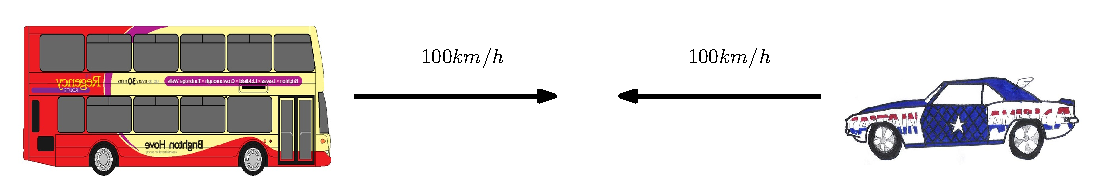
\includegraphics[width=9.25cm]{./Math_vector/movingVehicles.eps} \\
{\tiny 동일한 속력으로 서로 마주 보며 달리는 차량의 속도 }
\end{tabular}
\end{figure}
\end{frame}
%%%%%%%%%%%%%%%%%%%%%%%%%%%%%%%%%%%%%%%%%%%%%%%%%%%%%%%%%

%%%%%%%%%%%%%%%%%%%%%%%%%%%%%%%%%%%%%%%%%%%%%%%%%%%%%%%%%
\begin{frame}{화살표를 이용한 벡터 표현}
\begin{itemize}
\item 벡터를 표현하는 가장 직관적인 방법은 화살표를 이용
\item 화살표: 시점(始點)과 종점(終點)으로 구성 
\item 화살표의 방향은 벡터의 방향을 시각적으로 표현하고, 화살표의 길이는 벡터의 크기를 시각적으로 표현
\end{itemize}

\begin{figure}
\begin{tabular}{c}
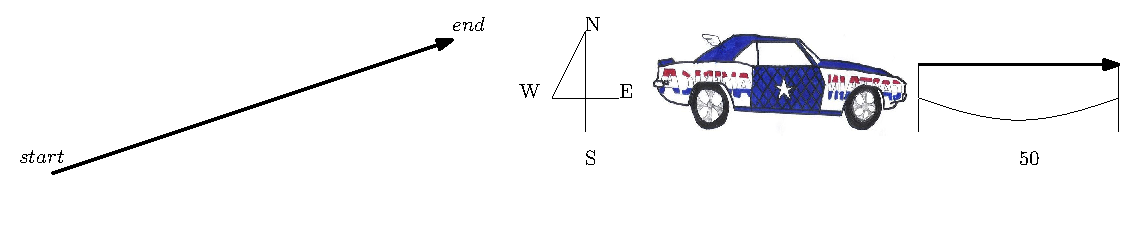
\includegraphics[width=8cm]{Math_vector/vectorExpression.eps}\\
{\tiny 벡터의 시각적 표현과 달리는 자동차 속도 표현의 예}
\end{tabular}
\end{figure}

\begin{figure}
\begin{tabular}{c}
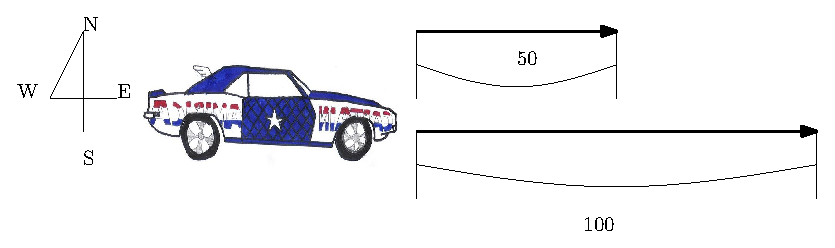
\includegraphics[width=8cm]{Math_vector/increasedSpeed.eps}\\
{\tiny 속력이 두 배로 늘어난 자동차의 속도}
\end{tabular}
\end{figure}

\end{frame}
%%%%%%%%%%%%%%%%%%%%%%%%%%%%%%%%%%%%%%%%%%%%%%%%%%%%%%%%%

%%%%%%%%%%%%%%%%%%%%%%%%%%%%%%%%%%%%%%%%%%%%%%%%%%%%%%%%%
\begin{frame}{동등벡터(equivalent vector)}

\begin{itemize}
\item 벡터의 표기법
\begin{itemize}
\item $\vec{a}$, $\mathbf a$
\end{itemize}
\end{itemize}

\begin{itemize}
\item 동등벡터
\begin{itemize}
\item 크기와 방향이 같으면 모두 동등한 벡터로 간주
\end{itemize}
\end{itemize}

\begin{figure}
\begin{tabular}{c}
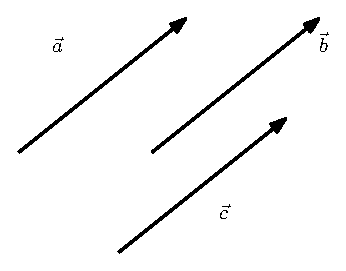
\includegraphics[width=5cm]{Math_vector/equivalentVectors.eps}\\
{\tiny 동등벡터}
\end{tabular}
\end{figure}

\end{frame}
%%%%%%%%%%%%%%%%%%%%%%%%%%%%%%%%%%%%%%%%%%%%%%%%%%%%%%%%%

%%%%%%%%%%%%%%%%%%%%%%%%%%%%%%%%%%%%%%%%%%%%%%%%%%%%%%%%%
\begin{frame}{동등벡터 찾기}

\begin{figure}
\begin{tabular}{c}
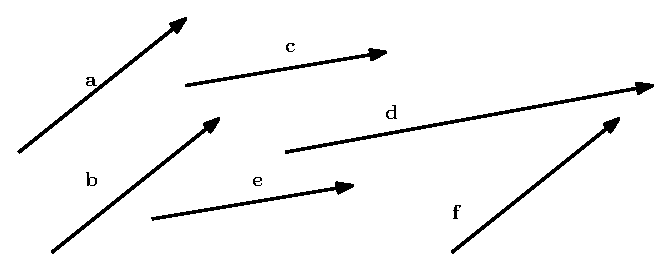
\includegraphics[width=10cm]{./Math_vector/equivalentVectors2.eps}\\
{\tiny 동등벡터 찾기}
\end{tabular}
\end{figure}

\end{frame}
%%%%%%%%%%%%%%%%%%%%%%%%%%%%%%%%%%%%%%%%%%%%%%%%%%%%%%%%%

%%%%%%%%%%%%%%%%%%%%%%%%%%%%%%%%%%%%%%%%%%%%%%%%%%%%%%%%%
\begin{frame}{벡터의 수학적 표현}

\begin{itemize}
\item 벡터: 화살표가 그려지는 공간의 차원(次元,dimension)에 따라 결정되는 개수의 성분
	\begin{itemize}
	\item $n$-튜플(tuple)
	\item $\mathbf v = ( v_1 , v_2 , v_3, \cdots , v_n )$
	\item $n$ 개의 차원을 가진 공간에서 그려지는 화살표 = $n$차원 벡터
	\end{itemize}
\end{itemize}

\end{frame}
%%%%%%%%%%%%%%%%%%%%%%%%%%%%%%%%%%%%%%%%%%%%%%%%%%%%%%%%%


%%%%%%%%%%%%%%%%%%%%%%%%%%%%%%%%%%%%%%%%%%%%%%%%%%%%%%%%%
\begin{frame}{2차원 벡터}

\begin{figure}[h!]
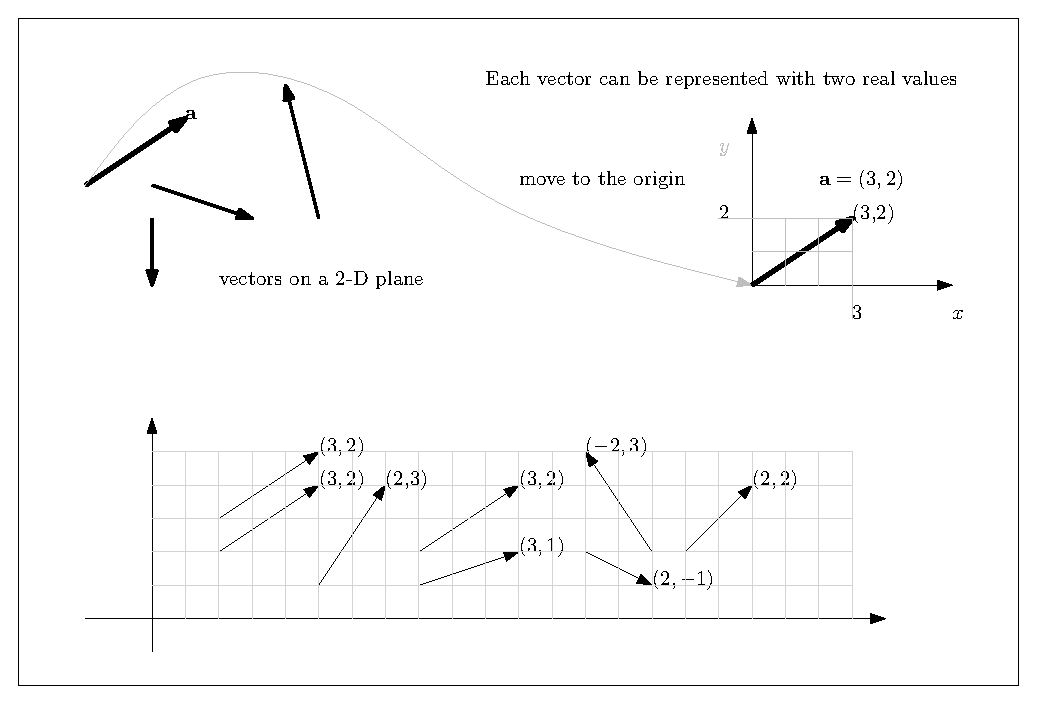
\includegraphics[width=10cm]{Math_vector/2dVectors.eps}
\end{figure}
\end{frame}
%%%%%%%%%%%%%%%%%%%%%%%%%%%%%%%%%%%%%%%%%%%%%%%%%%%%%%%%%


%%%%%%%%%%%%%%%%%%%%%%%%%%%%%%%%%%%%%%%%%%%%%%%%%%%%%%%%%
\begin{frame}{시점을 원점으로 옮기기}
시점이 원점이 아닌 벡터는 시점을 원점으로 끌어 오면 된다.
벡터의 시점은 (3,6)의 좌표에 놓여있고, 끝점은 (16,9)이다. 시작점을 원점으로 옮기는 것은 (-3,-6) 만큼의 이동을 하는 것이다.
따라서 끝점은 (13,3)의 위치로 이동하게 된다. 그러므로 이 벡터는 (13,3)으로 표현된다.

\begin{figure}
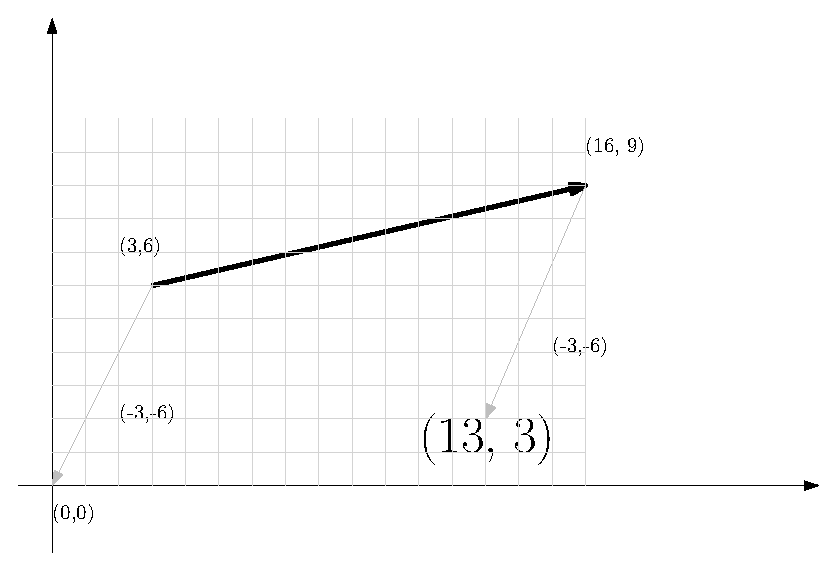
\includegraphics[width=9cm]{Math_vector/vectorMove.eps}
\end{figure}

\end{frame}
%%%%%%%%%%%%%%%%%%%%%%%%%%%%%%%%%%%%%%%%%%%%%%%%%%%%%%%%%

%%%%%%%%%%%%%%%%%%%%%%%%%%%%%%%%%%%%%%%%%%%%%%%%%%%%%%%%%
\begin{frame}{3차원 벡터}
3차원 벡터는 지금까지 살펴본 2차원 벡터에 축(軸, axis)을 하나 더하기만 하면 된다.
\begin{figure}
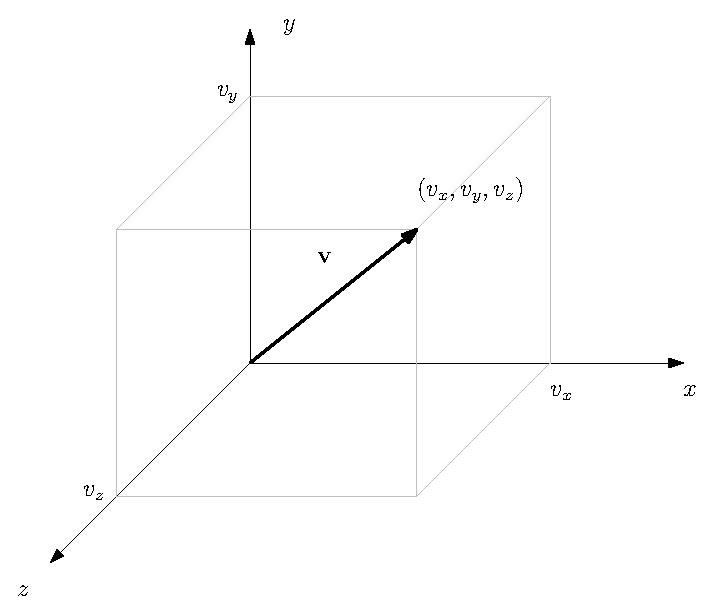
\includegraphics[width=9cm]{Math_vector/3dVector.eps}
\end{figure}
\end{frame}
%%%%%%%%%%%%%%%%%%%%%%%%%%%%%%%%%%%%%%%%%%%%%%%%%%%%%%%%%


%%%%%%%%%%%%%%%%%%%%%%%%%%%%%%%%%%%%%%%%%%%%%%%%%%%%%%%%%
\begin{frame}{벡터의 크기}
\begin{figure}
\begin{tabular}{p{6cm}p{5cm}}
\raisebox{-\totalheight}{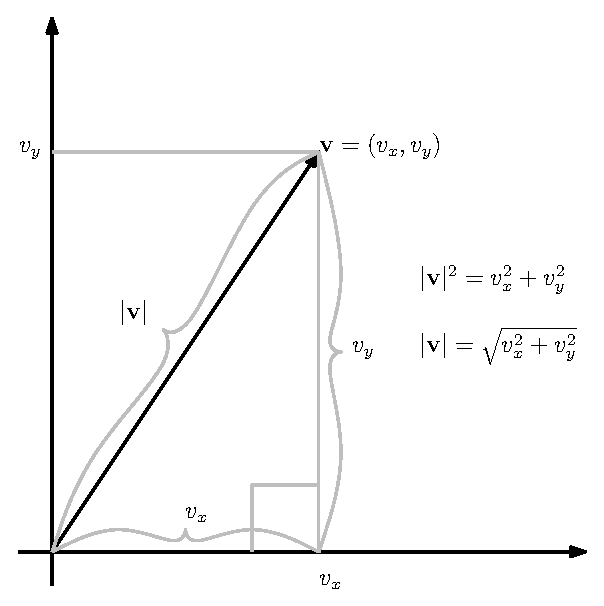
\includegraphics[width=6cm]{Math_vector/Pythagoras2D.eps}}
&
어떤 벡터 $\mathbf v$가 $(v_x , v_y )$로 표현될 때 
이 벡터의 크기는 $v_x$와 $v_y$로 어떻게 구할 수 있을까?
그 값은 '길이'에 대한 상식적 정의에 따라, 스칼라 값이며 양(陽, positive)의 값이 된다.
이렇게 양의 길이(positive length)를 벡터에 할당하는 것을 놈(norm)이라 하며, 
어떤 벡터 $\mathbf v$의 놈은 $|| \mathbf v ||$로 표현한다.
유클리드 기하에 의해 얻어지는 길이는 Euclidean Norm이라고 한다.
이는 피타고라스의 정리를 이용하여 쉽게 구할 수 있다.
\end{tabular}
\end{figure}
\end{frame}
%%%%%%%%%%%%%%%%%%%%%%%%%%%%%%%%%%%%%%%%%%%%%%%%%%%%%%%%%

%%%%%%%%%%%%%%%%%%%%%%%%%%%%%%%%%%%%%%%%%%%%%%%%%%%%%%%%%
\begin{frame}{3차원 벡터의 크기}
\begin{eqnarray}
\mathbf v = (v_x , v_y, v_z) \nonumber \\
|| \mathbf v || = \sqrt{v_x^2 + v_y^2 + v_z^2} \nonumber
\end{eqnarray}

\begin{figure}
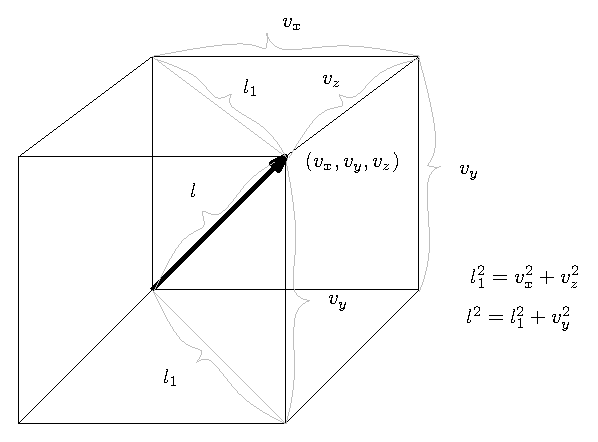
\includegraphics[width=7cm]{Math_vector/3dVectorLength.eps}
\end{figure}

\end{frame}
%%%%%%%%%%%%%%%%%%%%%%%%%%%%%%%%%%%%%%%%%%%%%%%%%%%%%%%%%


%%%%%%%%%%%%%%%%%%%%%%%%%%%%%%%%%%%%%%%%%%%%%%%%%%%%%%%%%
\begin{frame}{벡터의 정규화}
\begin{itemize}
	\item 정규화
	\begin{itemize}
	\item 단위 벡터는 길이가 1인 벡터.
	\item 어떤 벡터의 방향과 일치하는 단위벡터를 구하는 작업은 종종 많은 응용에서 필요.
	\item 이러한 작업은 벡터의 길이를 1로 만드는 것과 같다.
	\item 이를 정규화(normalization)이라고 한다.
	\end{itemize}
\end{itemize}

\begin{figure}
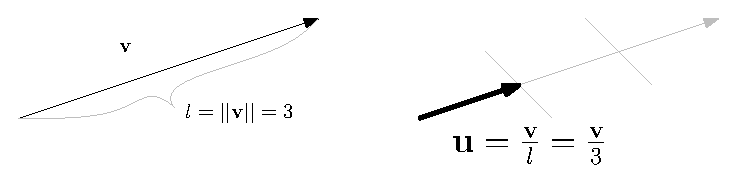
\includegraphics[width=8cm]{Math_vector/unitVector.eps}
\end{figure}
\end{frame}
%%%%%%%%%%%%%%%%%%%%%%%%%%%%%%%%%%%%%%%%%%%%%%%%%%%%%%%%%



%%%%%%%%%%%%%%%%%%%%%%%%%%%%%%%%%%%%%%%%%%%%%%%%%%%%%%%%%
\begin{frame}{벡터의 덧셈}
$\mathbf v + \mathbf w = (v_x + w_x, v_y + w_y , v_z + w_z )$
\begin{figure}
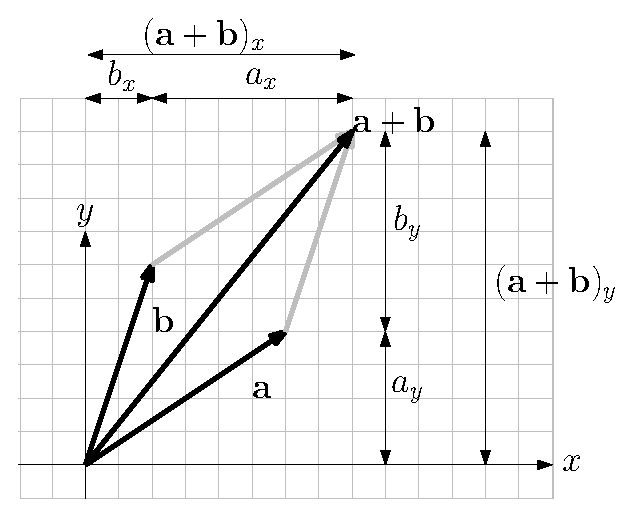
\includegraphics[width=8cm]{Math_vector/vectorAdd.eps}
\end{figure}
\end{frame}
%%%%%%%%%%%%%%%%%%%%%%%%%%%%%%%%%%%%%%%%%%%%%%%%%%%%%%%%%

%%%%%%%%%%%%%%%%%%%%%%%%%%%%%%%%%%%%%%%%%%%%%%%%%%%%%%%%%
\begin{frame}{벡터의 뺄셈}
$\mathbf v - \mathbf w = (v_x - w_x, v_y - w_y , v_z - w_z )$
\\

\begin{figure}
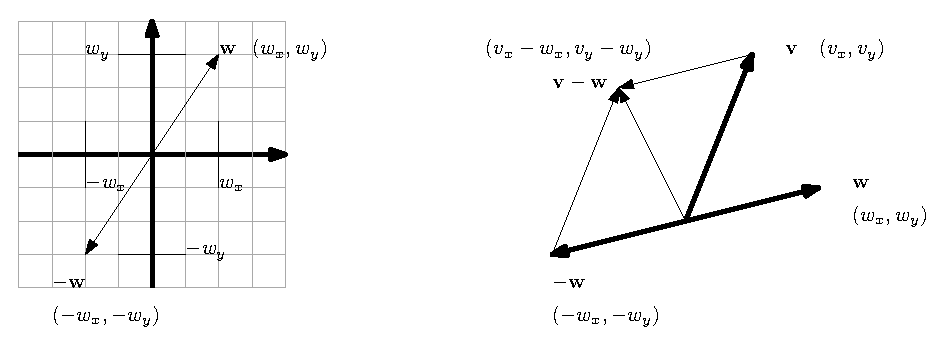
\includegraphics[width=12cm]{Math_vector/vectorSub.eps}
\end{figure}
\end{frame}
%%%%%%%%%%%%%%%%%%%%%%%%%%%%%%%%%%%%%%%%%%%%%%%%%%%%%%%%%

%%%%%%%%%%%%%%%%%%%%%%%%%%%%%%%%%%%%%%%%%%%%%%%%%%%%%%%%%
\begin{frame}{벡터에 스칼라 곱하기}

벡터는 크기만을 가진 스칼라와 곱할 수 있다. 어떤 스칼라 값 $s$가 있다고 하자, 이 스칼라 값과 벡터 $\mathbf v = (v_x , v_y, v_z)$를 곱한 $s \mathbf v$는 다음과 같다.
$$ s \mathbf v = (s v_x , s v_y , s v_z )$$
\end{frame}
%%%%%%%%%%%%%%%%%%%%%%%%%%%%%%%%%%%%%%%%%%%%%%%%%%%%%%%%%

%%%%%%%%%%%%%%%%%%%%%%%%%%%%%%%%%%%%%%%%%%%%%%%%%%%%%%%%%
\begin{frame}{벡터의 기본적인 연산 규칙}

\begin{eqnarray}
\mathbf a + \mathbf b = \mathbf b + \mathbf a \nonumber \\
(\mathbf a + \mathbf b) + \mathbf c = \mathbf a + (\mathbf b + \mathbf c) \nonumber \\
\mathbf a + \vec{0} = \vec{0} + \mathbf a = \mathbf a \nonumber \\
\mathbf a + (- \mathbf a) = \mathbf a - \mathbf a = \vec{0} \nonumber \\
(k+l) \mathbf a = k \mathbf a + l \mathbf a \nonumber \\
(kl) \mathbf a = k (l \mathbf a) \nonumber \\
1 \mathbf a = \mathbf a \nonumber \\
0 \mathbf a = \vec{0} \nonumber \\
(-1) \mathbf a = - \mathbf a \nonumber
\end{eqnarray}
\end{frame}
%%%%%%%%%%%%%%%%%%%%%%%%%%%%%%%%%%%%%%%%%%%%%%%%%%%%%%%%%

%%%%%%%%%%%%%%%%%%%%%%%%%%%%%%%%%%%%%%%%%%%%%%%%%%%%%%%%%
\begin{frame}{벡터의 스칼라 곱, 혹은 내적(dot product)}
\begin{itemize}
\item 내적
	\begin{itemize}
	\item 스칼라 곱(scalar product)라고도 부름 
	\item 두 개의 벡터를 피연산자(operand)로 하는 이항 연산(binary operator)로서 그 결과가 스칼라 값
	\item 두 벡터 $\mathbf a$와 $\mathbf b$의 내적은 $\mathbf a \cdot \mathbf b$로 표현
	\item 두 벡터가 이루는 사잇각이 $\theta$라고 하며, 내적의 크기는 다음과 같다.
		\begin{itemize}
		\item $\mathbf a \cdot \mathbf b = || \mathbf a || ||\mathbf b || \cos \theta$
		\end{itemize}
	\item 실제 계산 방법
		\begin{itemize}
		\item $\mathbf a , \mathbf b \in \mathbb R^n $
		\item $\mathbf a \cdot \mathbf b = a_1 b_1 + a_2 b_2 + \cdots + a_n b_n = \sum_{i=1}^n a_i b_i $
		\end{itemize}
	\end{itemize}
\end{itemize}

\end{frame}
%%%%%%%%%%%%%%%%%%%%%%%%%%%%%%%%%%%%%%%%%%%%%%%%%%%%%%%%%

%%%%%%%%%%%%%%%%%%%%%%%%%%%%%%%%%%%%%%%%%%%%%%%%%%%%%%%%%
\begin{frame}{벡터 내적의 의미}
\begin{figure}
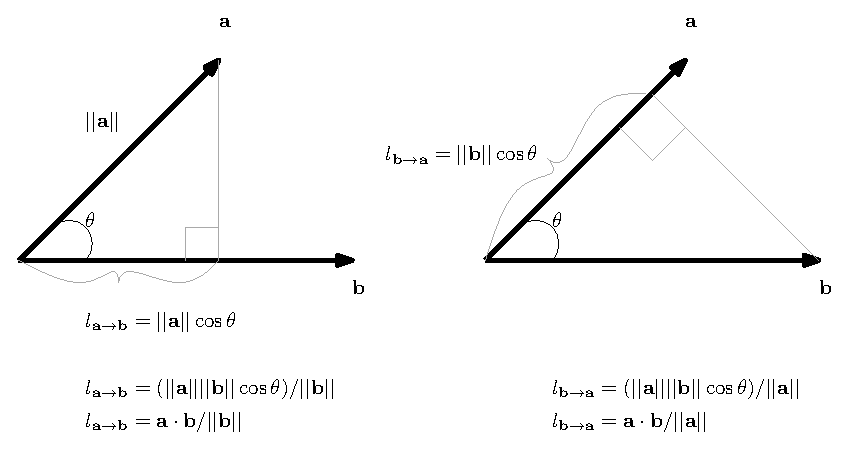
\includegraphics[width=12cm]{Math_vector/innerProduct.eps}
\end{figure}

\end{frame}
%%%%%%%%%%%%%%%%%%%%%%%%%%%%%%%%%%%%%%%%%%%%%%%%%%%%%%%%%


%%%%%%%%%%%%%%%%%%%%%%%%%%%%%%%%%%%%%%%%%%%%%%%%%%%%%%%%%
\begin{frame}{벡터 내적의 활용}
\begin{itemize}
\item 코사인 함수의 특성을 통해 간단히 얻어지는 사실
	\begin{itemize}
	\item $\theta = 0 \Rightarrow \cos \theta = 1 , \mathbf a \cdot \mathbf b = ||\mathbf a|| ||\mathbf b|| $
	\item $\theta = \pi / 2 \Rightarrow \cos \theta = 0, \mathbf a \cdot \mathbf b = 0 $
	\item $\mathbf a \cdot \mathbf a =  ||\mathbf a||^2$
	\end{itemize}
\end{itemize}


\begin{itemize}
\item 벡터를 이용하여 각도를 계산하거나 투영을 계산하는 데에 널리 사용
	\begin{itemize}
	\item $ \mathbf v \cdot \mathbf w  =  ||\mathbf v|| ||\mathbf w|| \cos \theta $
	\item $ \cos \theta = \frac{\mathbf v \cdot \mathbf w}{||\mathbf v||||\mathbf w||} $
	\item $ \theta  = \cos^{-1} \frac{\mathbf v \cdot \mathbf w}{||\mathbf v||||\mathbf w||} $
	\item $ \theta =  \cos^{-1}\frac{ v_x w_x + v_y w_y + v_z w_y}{\sqrt{v_x^2 + v_y^2 + v_z^2} \sqrt{w_x^2 + w_y^2 + w_z^2} }$
	\end{itemize} 
\end{itemize}

\end{frame}
%%%%%%%%%%%%%%%%%%%%%%%%%%%%%%%%%%%%%%%%%%%%%%%%%%%%%%%%%


%%%%%%%%%%%%%%%%%%%%%%%%%%%%%%%%%%%%%%%%%%%%%%%%%%%%%%%%%
\begin{frame}{벡터 내적의 활용}
\hrule

\noindent \colorbox{lightgray}{\begin{minipage}{6cm}예제\end{minipage}} 


\noindent 어떤 두 벡터가 각각 (3,2)와 (4,1)이라고 하자. 두 벡터가 이루는 각도를 구하라.

\noindent \colorbox{lightgray}{\begin{minipage}{6cm}정답\end{minipage}} 

\noindent 두 벡터를 각각 $\mathbf v$와 $\mathbf w$로 표현하자. 두 벡터의 내적 $\mathbf v \cdot \mathbf w$는 $3 \cdot 4 + 2 \cdot 1$, 즉 14이다.
각각의 길이는 $||\mathbf v|| = \sqrt{9+4} = \sqrt{13}$과 $||\mathbf w|| = \sqrt{16+1} = \sqrt{17}$이다.
따라서 두 벡터의 사이각은 다음과 같다.
$$\theta = \cos^{-1} \frac{14}{\sqrt{13} \sqrt{17}} = \cos^{-1} \frac{14}{\sqrt{221}} \simeq \cos^{-1} 0.94174191159484 \simeq 19.65 ^{\circ}$$

\hrule

\end{frame}
%%%%%%%%%%%%%%%%%%%%%%%%%%%%%%%%%%%%%%%%%%%%%%%%%%%%%%%%%


%%%%%%%%%%%%%%%%%%%%%%%%%%%%%%%%%%%%%%%%%%%%%%%%%%%%%%%%%
\begin{frame}{좌표축과 좌표 - 1/3 기본 의미}

\begin{itemize}
\item $\mathbf a  = (k, l)$로 표현된다는 것은 $xy$ 좌표계에서 기저벡터가 되는
$x$축 단위벡터를 $\mathbf u$와 $y$축 단위벡터를 $\mathbf v$를 다음과 같이 합성한 것
\end{itemize}

\begin{figure}
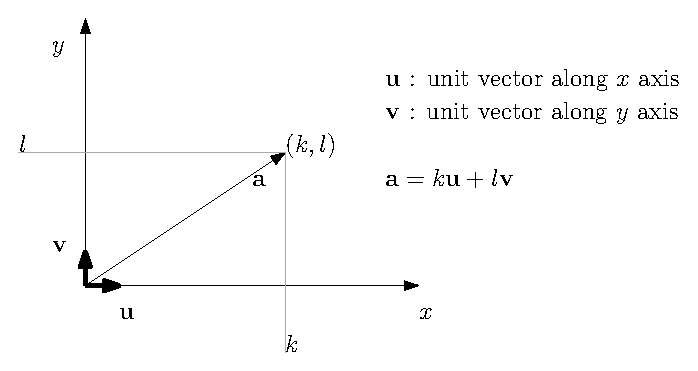
\includegraphics[width=10cm]{Math_vector/vectorComponents.eps}
\end{figure}

\end{frame}
%%%%%%%%%%%%%%%%%%%%%%%%%%%%%%%%%%%%%%%%%%%%%%%%%%%%%%%%%


%%%%%%%%%%%%%%%%%%%%%%%%%%%%%%%%%%%%%%%%%%%%%%%%%%%%%%%%%
\begin{frame}{좌표축과 좌표 - 2/3 새로운 축의 정의}

\begin{itemize}
\item 새로운 직교 좌표계를 고려해 보자. 여기서는 두 축이 $\mathbf u$와 $\mathbf v$
\item $\mathbf a$의 $\mathbf u$ 축 투영 길이 $\alpha$, $\mathbf v$ 축 투영 길이 $\beta$ 계산
\item 이 두 축을 기준으로 하는 좌표계에서는 $\mathbf a$가 $(\alpha, \beta)$의 좌표로 표현됨
\end{itemize}


\begin{figure}
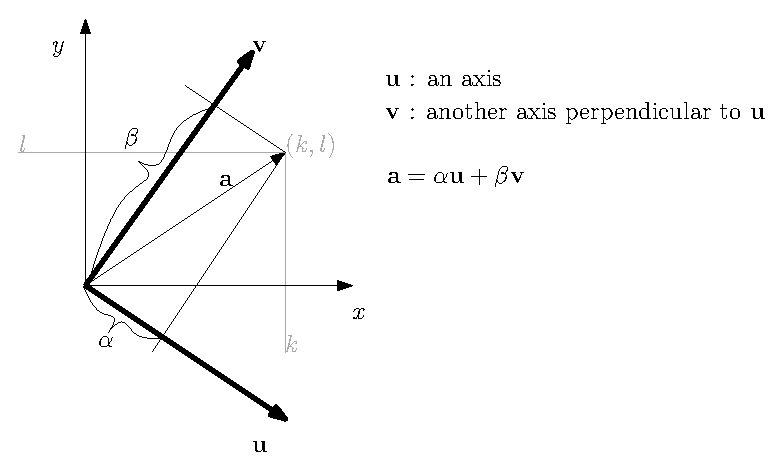
\includegraphics[width=10cm]{Math_vector/vectorComponentsArb.eps}
\end{figure}

\end{frame}
%%%%%%%%%%%%%%%%%%%%%%%%%%%%%%%%%%%%%%%%%%%%%%%%%%%%%%%%%

%%%%%%%%%%%%%%%%%%%%%%%%%%%%%%%%%%%%%%%%%%%%%%%%%%%%%%%%%
\begin{frame}{좌표축과 좌표 - 3/3 내적을 이용한 투영 길이 구하기}

\begin{itemize}
\item $\mathbf a$가 축 $\mathbf u$와 $\mathbf v$ 방향으로 가지는 길이 $\alpha$와 $\beta$는 어떻게 구하나
	\begin{itemize}
	\item 내적을 이용
	\item $\alpha$는 $\mathbf a$를 $\mathbf u$ 방향으로 투영한 그림자의 길이 =  $\mathbf a \cdot \mathbf u / || \mathbf u ||$
	\item 축은 단위 벡터로 표현하므로 $||\mathbf u||=1$. 따라서 $\alpha = \mathbf a \cdot \mathbf u$
	\item 비슷한 방법으로 $\beta = \mathbf a \cdot \mathbf v$
	\item $\mathbf u$와 $\mathbf v$를 축으로 하는 좌표계에서 $\mathbf a$는 $(\mathbf a \cdot \mathbf u, \mathbf a \cdot \mathbf v)$
	\end{itemize}
\end{itemize}

\begin{figure}
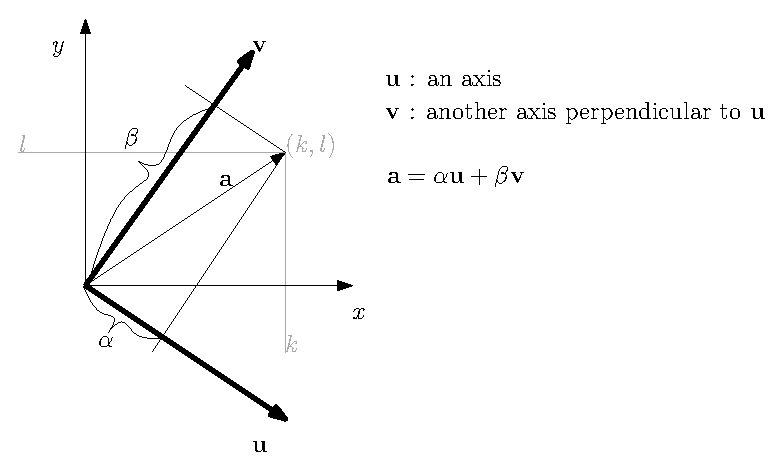
\includegraphics[width=6cm]{Math_vector/vectorComponentsArb.eps}
\end{figure}

\end{frame}
%%%%%%%%%%%%%%%%%%%%%%%%%%%%%%%%%%%%%%%%%%%%%%%%%%%%%%%%%


%%%%%%%%%%%%%%%%%%%%%%%%%%%%%%%%%%%%%%%%%%%%%%%%%%%%%%%%%
\begin{frame}{새로운 좌표축의 정의}

\hrule
\noindent \colorbox{lightgray}{\begin{minipage}{6cm}예제\end{minipage}} 


\noindent 그림처럼 어떤 벡터 $\mathbf a$가 (4,5)이고, 다른 벡터 $\mathbf b$는 (10,2)라고 하자.
이때 벡터 $\mathbf a$를 $\mathbf b$ 위에 수직방향으로 내린 그림자가 되는 벡터 $\mathbf a_{prj}$을 구하라.

\begin{figure}
    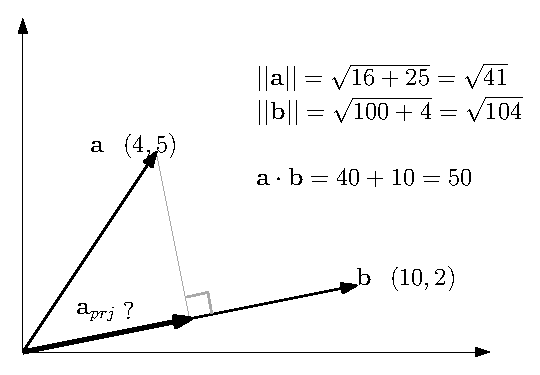
\includegraphics[width=4cm]{Math_vector/vecProjection.eps}
\end{figure}

\noindent \colorbox{lightgray}{\begin{minipage}{6cm}정답\end{minipage}} 

$$l = \mathbf a \cdot \mathbf b / || \mathbf b||$$
$$\mathbf a_{prj} = l \tilde{\mathbf b} = \frac{50}{104} (10,2)  \simeq  (4.8, 0.96) $$

\hrule

\end{frame}
%%%%%%%%%%%%%%%%%%%%%%%%%%%%%%%%%%%%%%%%%%%%%%%%%%%%%%%%%

%%%%%%%%%%%%%%%%%%%%%%%%%%%%%%%%%%%%%%%%%%%%%%%%%%%%%%%%%
\begin{frame}{벡터의 외적(外積) - 의미}

\begin{itemize}
\item 벡터의 외적(cross product)
	\begin{itemize}
	\item 벡터 곱(vector product): 두 벡터를 피연산자로 하는 이항연산으로 그 결과가 벡터
	\item 벡터를 곱해 행렬을 얻는 외적(outer product)과 용어의 혼동이 있음. 여기서는 결과가 벡터인 곱
	\end{itemize}
\item 표현
	\begin{itemize}
	\item 두 벡터 $\mathbf a$와 $\mathbf b$의 외적은 $\mathbf a \times \mathbf b$로 표현
	\item 그 결과는 벡터이므로 $k \mathbf n$ ($\mathbf n$은 $\mathbf a$와 $\mathbf b$에 동시에 수직인 단위벡터)
	\item 동시에 수직인 벡터는 두 개가 존재. 좌표계에 의해 결정됨.
	\end{itemize}
\end{itemize}

\begin{figure}
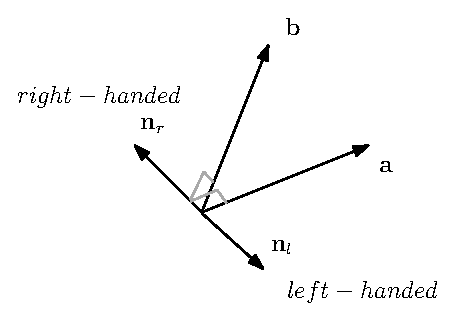
\includegraphics[width=5cm]{Math_vector/crossProductDir.eps}
\end{figure}

\end{frame}
%%%%%%%%%%%%%%%%%%%%%%%%%%%%%%%%%%%%%%%%%%%%%%%%%%%%%%%%%


%%%%%%%%%%%%%%%%%%%%%%%%%%%%%%%%%%%%%%%%%%%%%%%%%%%%%%%%%
\begin{frame}{벡터의 외적(外積) 의미의 수학적 표현}

\begin{itemize}
\item 두 벡터의 외적
	\begin{itemize}
	\item 외적의 크기 $k$
		\begin{itemize}
		\item 두 벡터의 크기와 사잇각의 사인(sine) 값에 비례
		\item $k = ||\mathbf a|| |\mathbf b|| \sin \theta$
		\end{itemize}
	\item 외적의 방향 $\mathbf n$
		\begin{itemize}
		\item $\mathbf n$: 두 벡터에 수직인 방향 벡터
		\end{itemize}
	\end{itemize}
\item 따라서 두 벡터의 외적은 다음과 같이 표현할 수 있다.
	\begin{itemize}
	\item $\mathbf a \times \mathbf b = ||\mathbf a|| |\mathbf b|| \sin \theta \mathbf n$
	\end{itemize}
\end{itemize}


\end{frame}
%%%%%%%%%%%%%%%%%%%%%%%%%%%%%%%%%%%%%%%%%%%%%%%%%%%%%%%%%

%%%%%%%%%%%%%%%%%%%%%%%%%%%%%%%%%%%%%%%%%%%%%%%%%%%%%%%%%
\begin{frame}{외적이 가진 의미}

\begin{itemize}
\item 외적을 표현하는 식 $\mathbf a \times \mathbf b = ||\mathbf a|| |\mathbf b|| \sin \theta \mathbf n$의 의미
	\begin{itemize}
	\item 외적은 두 벡터에 동시에 수직한 벡터
	\item 크기는 두 벡터가 수직일 때에 최대, 같은 방향이나 반대방향일 때 최소
	\item 외적의 크기는 벡터 $\mathbf a$와 $\mathbf b$의 끝점을 연결한 삼각형의 넓이 $S$에 비례
		\begin{itemize}
		\item $|| \mathbf a \times \mathbf b || = 2 S $
		\end{itemize}
		\end{itemize}
\end{itemize}


\begin{figure}
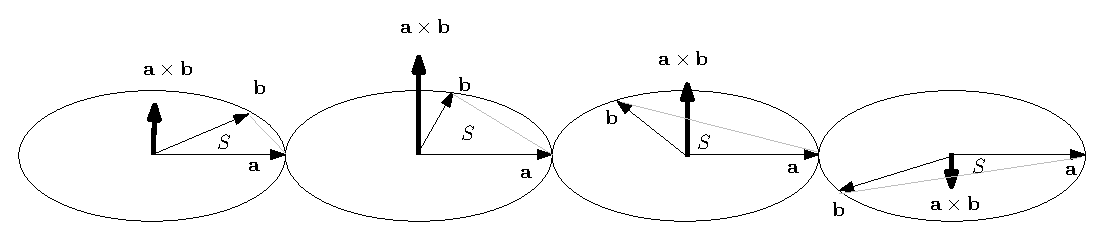
\includegraphics[width=12cm]{Math_vector/crossProductDirSize.eps}
\end{figure}

\end{frame}

%%%%%%%%%%%%%%%%%%%%%%%%%%%%%%%%%%%%%%%%%%%%%%%%%%%%%%%%%


%%%%%%%%%%%%%%%%%%%%%%%%%%%%%%%%%%%%%%%%%%%%%%%%%%%%%%%%%
\begin{frame}{외적의 계산}

\begin{itemize}
\item 3차원 벡터의 외적을 구하기
	\begin{itemize}
	\item $\mathbf a=(a_1, a_2, a_3), \mathbf b=(b_1, b_2, b_3)$
	\item 두 벡터의 외적: $\mathbf a \times \mathbf b = (a_2 b_3 - a_3 b_2, a_3 b_1 - a_1 b_3, a_1 b_2 - a_2 b_1)$
	\end{itemize}
\item ``행렬"을 이용한 곱셈으로 구하기
	\begin{itemize}
	\item ``반대칭(skew-symmetric 혹은 antisymmetric)" 행렬 이용
	\end{itemize}
\end{itemize}

\begin{eqnarray}
\mathbf A^* = \left ( 
\begin{array}{ccc}
0 & -a_3 & a_2 \\
a_3 & 0 & -a_1 \\
-a_2 & a_1 & 0 \nonumber
\end{array}
\right ) \nonumber
\end{eqnarray}

\begin{eqnarray}
\mathbf A^* \mathbf b = \left ( 
\begin{array}{ccc}
0 & -a_3 & a_2 \\
a_3 & 0 & -a_1 \\
-a_2 & a_1 & 0
\end{array}
\right ) \mathbf b
= (a_2 b_3 - a_3 b_2, a_3 b_1 - a_1 b_3, a_1 b_2 - a_2 b_1 ) \nonumber
\end{eqnarray}

\end{frame}

%%%%%%%%%%%%%%%%%%%%%%%%%%%%%%%%%%%%%%%%%%%%%%%%%%%%%%%%%


%%%%%%%%%%%%%%%%%%%%%%%%%%%%%%%%%%%%%%%%%%%%%%%%%%%%%%%%%
\begin{frame}{외적의 연산 법칙들}

\begin{eqnarray}\nonumber
\mathbf a \times \mathbf b = - \mathbf b \times \mathbf a \\ \nonumber
\mathbf a \times ( \mathbf b \times \mathbf c) = (\mathbf a \times \mathbf b) \times \mathbf c \\ \nonumber
(\mathbf a + \mathbf b ) \times \mathbf c = (\mathbf a \times \mathbf c) + (\mathbf b \times \mathbf c) \\ \nonumber
k(\mathbf a \times \mathbf b) = k \mathbf a \times \mathbf b = \mathbf a \times k \mathbf b \\ \nonumber
\mathbf a \times \vec{0} = \vec{0} \times \mathbf a = \vec{0} \\ \nonumber
\mathbf a \times \mathbf a = \vec{0} \\ \nonumber
\mathbf a \cdot (  \mathbf a \times \mathbf b) = \vec{0} \\ \nonumber
\mathbf b \cdot ( \mathbf a \times \mathbf b) = \vec{0}
\end{eqnarray}

\end{frame}
%%%%%%%%%%%%%%%%%%%%%%%%%%%%%%%%%%%%%%%%%%%%%%%%%%%%%%%%%


%%%%%%%%%%%%%%%%%%%%%%%%%%%%%%%%%%%%%%%%%%%%%%%%%%%%%%%%%
\begin{frame}{2차원 공간에서의 외적과 외적의 응용}

\begin{itemize}
\item 2차원 공간의 두 벡터 $\mathbf a=(a_x, a_y)$와 $\mathbf b=(b_x, b_y)$의 외적은?
	\begin{itemize}
	\item 그림의 회색 면은 2차원 공간의 일부
	\item 두 벡터 $\mathbf a$와 $\mathbf b$의 외적은 2차원 공간 밖에서 정의
	\item 축 $z$가 필요하며, 이 $z$ 축 성분으로만 표현
	\end{itemize}
\end{itemize}

\begin{figure}
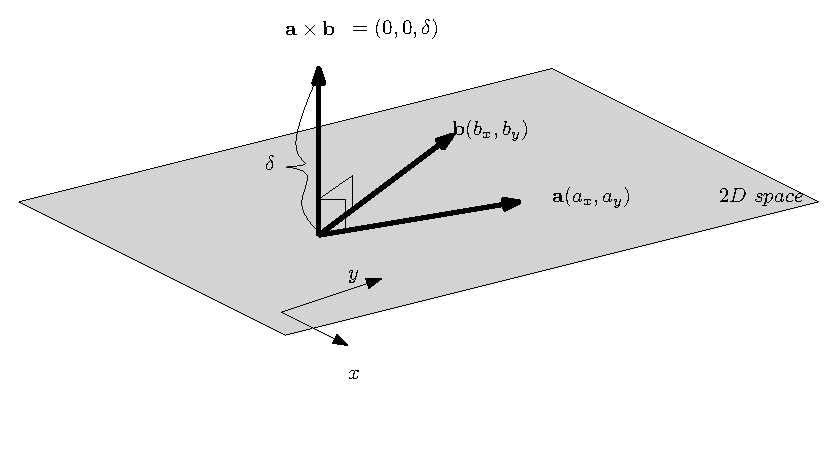
\includegraphics[width=12cm]{Math_vector/crossProduct2D.eps}
\end{figure}

\end{frame}
%%%%%%%%%%%%%%%%%%%%%%%%%%%%%%%%%%%%%%%%%%%%%%%%%%%%%%%%%


%%%%%%%%%%%%%%%%%%%%%%%%%%%%%%%%%%%%%%%%%%%%%%%%%%%%%%%%%
\begin{frame}{2차원 공간에서의 외적과 외적의 응용}
\begin{itemize}
\item 2차원 벡터의 외적이 2차원 공간 밖에 정의가 되고, 이것은 3차원 벡터라고 볼 수 있다.
\item 2차원 벡터 $\mathbf a = (a_x, a_y)$와 $\mathbf b= (b_x, b_y)$를 3차원 벡터로 가정
	\begin{itemize}
	\item $\mathbf a = (a_x , a_y, 0)$
	\item $\mathbf b = (b_x , b_y, 0)$
	\item $\mathbf a \times \mathbf b = (0, 0, a_x b_y - a_y b_x )$
	\end{itemize}
\end{itemize}

\begin{itemize}
\item $z$ 성분의 값으로 알 수 있는 것들  (이를 $\delta$라고 하자) 
	\begin{itemize}
	\item $\delta>0$인 경우는 $\mathbf b$가 $\mathbf a$의 진행 방향을 기준으로 왼쪽에 있음
	\item $\delta<0$인 경우는 오른쪽
	\item 절대값은 두 벡터 사이에 만들어지는 삼각형의 크기에 비례
	\end{itemize}
\end{itemize}

\end{frame}
%%%%%%%%%%%%%%%%%%%%%%%%%%%%%%%%%%%%%%%%%%%%%%%%%%%%%%%%%


%%%%%%%%%%%%%%%%%%%%%%%%%%%%%%%%%%%%%%%%%%%%%%%%%%%%%%%%%
\begin{frame}{삼각형 넓이 구하기}

\hrule
\noindent \colorbox{lightgray}{\begin{minipage}{6cm}예제\end{minipage}} 

\noindent 꼭지점 좌표가 (2,1), (8,4), (4,8)인 삼각형의 넓이 $S$를 구하라.

\noindent \colorbox{lightgray}{\begin{minipage}{6cm}정답\end{minipage}} 

{\small 꼭지점들을 각각 $\mathbf a, \mathbf b, \mathbf c$로 표현하자.
우리는 $\mathbf a$에서 $\mathbf b$로 가는 벡터를 구할 수 있고, $\mathbf u = (6,3)$가 된다.
비슷한 방식으로 $\mathbf a$에서 $\mathbf c$로 가는 벡터는 $\mathbf v = (2,7)$이다.
삼각형의 넓이는 이 두 벡터의 외적이 가지는 크기의 반이다.}

$$S = \frac{1}{2} ||\mathbf a \times \mathbf b || = \frac{6 \cdot 7 - 3 \cdot 2}{2} = 18$$

\begin{figure}
    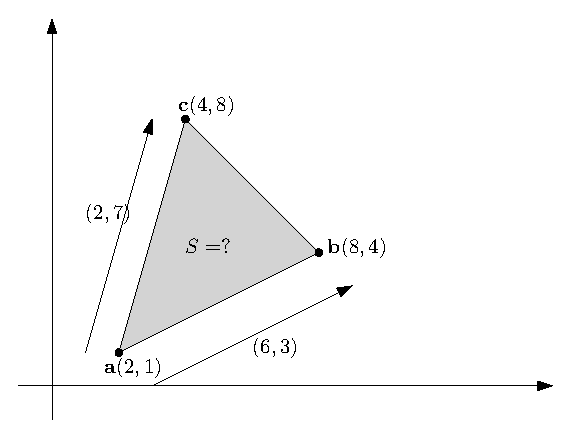
\includegraphics[width=4cm]{Math_vector/triangleArea.eps}
\end{figure}

\hrule

\end{frame}
%%%%%%%%%%%%%%%%%%%%%%%%%%%%%%%%%%%%%%%%%%%%%%%%%%%%%%%%%

%%%%%%%%%%%%%%%%%%%%%%%%%%%%%%%%%%%%%%%%%%%%%%%%%%%%%%%%%
\begin{frame}{외적과 평면}

\begin{itemize}
\item 외적의 또 다른 응용
	\begin{itemize}
	\item 평면 표현
		\begin{itemize}
		\item 평면은 그 평면 위의 삼각형으로 표현 가능 = 3 개의 점 = 9 개의 원소
		\item 좀 더 효율적인 방법 = 법선 벡터를 이용하기
		\item 법선벡터 = 평면이 바라보는 방향을 나타내는 벡터
		\item 법선벡터가 나타내는 것은 하나의 평면이 아니라 동일한 방향을 쳐다보는 모든 평면
		\item 평면의 표현 = (법선벡터, 평면이 지나는 점) : 6 개의 원소로 표현 가능
		\item 법선벡터 구하기: 벡터의 외적을 이용
		\end{itemize}
	\end{itemize}
\end{itemize}

\end{frame}


%%%%%%%%%%%%%%%%%%%%%%%%%%%%%%%%%%%%%%%%%%%%%%%%%%%%%%%%%
\begin{frame}{행렬}

\begin{itemize}
\item 행렬의 역사
	\begin{itemize}
	\item 1차 방정식의 풀이에 아주 오래 전부터 사용
	\item 그 특성이 정확히 파악되지 않고 1800년대까지는 배열(array)이라는 이름으로 알려짐
	\item 기원전 10세기에서 기원전 2세기 사이에 여러 세대에 걸쳐 쓰여진 중국의 구장산술(九章算術)에 연립 방정식을 풀기 위해 소개
	\item 판별식의 개념 등장
	\item 1545년에야 이탈리아 수학자 지롤라모 카르다노(Girolamo Cardano)가 그의 저서 "위대한 기술(Ars Magna)"를 통해 유럽에 전함
	\item 오랜 기간 동안 많은 수학자들이 이 행렬을 다루며 다양한 성질을 발견
	\item 행렬은 공간을 나루는 데에 필요한 유용한 도구
	\item 공간 내의 점들을 이떤 위치에서 다른 위치로 옮겨 놓는 다양한 변환이 행렬을 이용하여 표현됨
	\end{itemize}
\end{itemize}

\end{frame}


%%%%%%%%%%%%%%%%%%%%%%%%%%%%%%%%%%%%%%%%%%%%%%%%%%%%%%%%%


%%%%%%%%%%%%%%%%%%%%%%%%%%%%%%%%%%%%%%%%%%%%%%%%%%%%%%%%%
\begin{frame}{행렬이란 무엇인가}

\begin{itemize}
\item 행렬은 2차원으로 배열된 수
\item 가로 줄을 행(row), 세로 줄을 열(column)
\item $m$ 개의 행과 $n$ 개의 열로 이루어진 행렬은 $\mathbf A$는 다음의 모양
\item $\mathbf A = \left [ 
\begin{array}{cccccc}
a_{11} & a_{12} & \cdots & a_{1j} & \cdots & a_{1n} \\
a_{21} & a_{22} & \cdots & a_{2j} & \cdots & a_{2n} \\
\vdots & \vdots & \ddots &   \vdots   & \ddots & \vdots \\
a_{i1} & a_{i2} & \cdots & a_{ij} & \cdots & a_{in} \\
\vdots & \vdots & \ddots & \vdots & \ddots & \vdots\\
a_{m1} & a_{m2} & \cdots & a_{mj} & \cdots & a_{mn} \\
\end{array}
\right ]$
\item $m \times n$ 행렬이라고 하며 $\mathbf A \in \mathbb R^{m\times n}$로 표현
\item 각 행은 $n$ 개의 원소를 가진 행벡터(row vector)
\item 각 열은 $m$ 개의 원소를 가진 열벡터(column vector)
\end{itemize}

\end{frame}


%%%%%%%%%%%%%%%%%%%%%%%%%%%%%%%%%%%%%%%%%%%%%%%%%%%%%%%%%


%%%%%%%%%%%%%%%%%%%%%%%%%%%%%%%%%%%%%%%%%%%%%%%%%%%%%%%%%
\begin{frame}{행벡터와 열벡터}
$\mathbf A$를 행벡터 $\mathbf v_i^r$로 표현하면 다음과 같다.
$\mathbf A = \left [ 
\begin{array}{c}
\mathbf v_1^r\\
\mathbf v_2^r\\
\vdots\\
\mathbf v_m^r
\end{array}
\right ]$

$\mathbf A$를 열벡터 $\mathbf v_j^c$로 표현하면 다음과 같다.
$\mathbf A = \left [ 
\begin{array}{cccc}
\mathbf v_1^c & \mathbf v_2^c & \cdots & \mathbf v_n^c
\end{array}
\right ]$

\begin{figure}
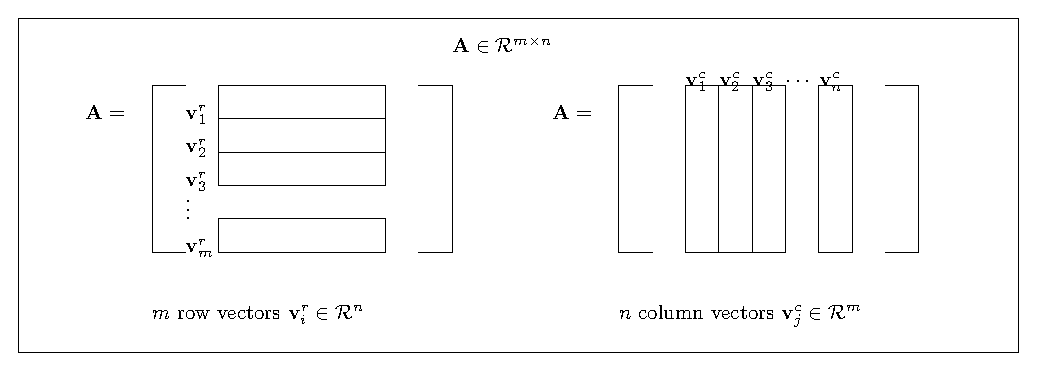
\includegraphics[width=12cm]{Math_matrix/matrixAsVectorCollection.eps}
\end{figure}

\end{frame}
%%%%%%%%%%%%%%%%%%%%%%%%%%%%%%%%%%%%%%%%%%%%%%%%%%%%%%%%%


%%%%%%%%%%%%%%%%%%%%%%%%%%%%%%%%%%%%%%%%%%%%%%%%%%%%%%%%%
\begin{frame}{정사각 행렬 - square matrix}

\begin{itemize}
\item 정방행렬, 혹은 정사각형 행렬은 행과 열의 수가 동일한 행렬.
	\begin{itemize}
	\item $\mathbf A \in \mathbb R^{n \times n}$인 행렬
	\item 정방행렬은 물리 문제에서 운동을 다루거나 그래픽스에서 변환을 다룰 때에 빈번히 나타남
	\end{itemize}
\item 다음 행렬 $\mathbf A$는 $3\times 3$의 정사각 행렬이다.
	\begin{itemize}
	\item $ \mathbf A = \left [ 
		\begin{array}{ccc}
		a_{11} & a_{12} & a_{13} \nonumber \\
		a_{21} & a_{22} & a_{23} \\
		a_{31} & a_{32} & a_{33} 
		\end{array}
		\right ] $
	\end{itemize}
\end{itemize}


\end{frame}
%%%%%%%%%%%%%%%%%%%%%%%%%%%%%%%%%%%%%%%%%%%%%%%%%%%%%%%%%


%%%%%%%%%%%%%%%%%%%%%%%%%%%%%%%%%%%%%%%%%%%%%%%%%%%%%%%%%
\begin{frame}{전치 행렬 - transpose}

\begin{itemize}
\item 어떤 행렬 $\mathbf A$의 전치행렬은 $\mathbf A^{\rm T}$
	\begin{itemize}
	\item $\mathbf B = \mathbf A^{\rm T} \Rightarrow b_{ij} = a_{ji}$
	\item 따라서, $m \times n$ 행렬의 전치는 $n \times m$ 행렬
	\item $\mathbf A \in \mathbb R^{m \times n} \Rightarrow \mathbf B \in \mathbb R^{n \times m}$
	\end{itemize}
\item 전치행렬의 성질
	\begin{itemize}
	\item $\mathbf (\mathbf A^{\rm T})^{\rm T} = A$
	\item $(\mathbf A + \mathbf B)^{\rm T} = \mathbf A^{\rm T} + \mathbf B^{\rm T}$
	\item $(k\mathbf A)^{\rm T} = k \mathbf A^{\rm T}$
	\item $(\mathbf {AB})^{\rm T} = \mathbf B^{\rm T} \mathbf A^{\rm T}$
	\end{itemize}
\item 그래픽스(graphics) 분야에서 매우 유용한 사용 방법은 회전 변환 행렬의 역행렬을 구할 때
\item 3차원 공간의 회전 변환은 정규직교(orthonormal) 특성
\item 정규직교 행렬의 역행렬은 그 행렬의 전치임이 알려져 있음
\end{itemize}

\end{frame}
%%%%%%%%%%%%%%%%%%%%%%%%%%%%%%%%%%%%%%%%%%%%%%%%%%%%%%%%%


%%%%%%%%%%%%%%%%%%%%%%%%%%%%%%%%%%%%%%%%%%%%%%%%%%%%%%%%%
\begin{frame}{대각 행렬 - diagonal matrix}

\begin{itemize}
\item 대각성분은 어떤 행렬 $\mathbf A$의 $i$ 행 $j$ 열 성분을 $a_{ij}$라고 표현할 때, $i=j$인 성분
\item 대각행렬은 대각성분을 제외한 다른 모든 성분의 값이 0인 행렬이다
	\begin{itemize}
	\item $\mathbf A = \left [ 
		\begin{array}{ccc}
		a_{11} & 0 & 0 \\
		0 & a_{22} & 0 \\
		0 & 0 & a_{33} \\
		\end{array}
		\right ]$
	\end{itemize}
\item 대각행렬을 다른 행렬과 곱했을 때의 성질
	\begin{itemize}
	\item 어떤 $3 \times 3$ 대각행렬을 $\mathbf D$, 1,2,3 행 대각성분은 $d_1, d_2, d_3$
	\item 다른 어떤 $3 \times 3$ 행렬 $\mathbf A$와 $\mathbf D$의 곱
		\begin{itemize}
		\item $\mathbf{DA} = \left [
			\begin{array}{ccc}
			d_1 a_{11} & d_1 a_{12} & d_1 a_{13} \\
			d_2 a_{21} & d_2 b_{22} & d_2 b_{23} \\
			d_3 a_{31} & d_3 b_{32} & d_3 b_{33} 
			\end{array}
			\right ]$
		\item 
		\item $\mathbf{AD} = \left [
			\begin{array}{ccc}
			d_1 a_{11} & d_2 a_{12} & d_3 a_{13} \\
			d_1 a_{21} & d_2 b_{22} & d_3 b_{23} \\
			d_1 a_{31} & d_2 b_{32} & d_3 b_{33}
			\end{array}
			\right ]$
		\end{itemize}
	\end{itemize}
\end{itemize}

\end{frame}
%%%%%%%%%%%%%%%%%%%%%%%%%%%%%%%%%%%%%%%%%%%%%%%%%%%%%%%%%


%%%%%%%%%%%%%%%%%%%%%%%%%%%%%%%%%%%%%%%%%%%%%%%%%%%%%%%%%
\begin{frame}{대각 행렬과 벡터의 곱 (1/2)}

대각행렬 $\mathbf D$와 열벡터 $\mathbf v \in \mathbb R^3$이 $(v_1, v_2, v_3)^{\rm T}$의 곱
$$
\mathbf {Dv} = 
\left [ 
\begin{array}{ccc}
a_{11} & 0 & 0 \\
0 & a_{22} & 0 \\
0 & 0 & a_{33} \\
\end{array}
\right ]
\left [
\begin{array}{c}
v_1 \\
v_2 \\
v_3 \\
\end{array}
\right ]
=
\left [
\begin{array}{c}
d_1 v_1 \\
d_2 v_2 \\
d_3 v_3 \\
\end{array}
\right ]
$$
\end{frame}
%%%%%%%%%%%%%%%%%%%%%%%%%%%%%%%%%%%%%%%%%%%%%%%%%%%%%%%%%


%%%%%%%%%%%%%%%%%%%%%%%%%%%%%%%%%%%%%%%%%%%%%%%%%%%%%%%%%
\begin{frame}{대각 행렬과 벡터의 곱 (2/2)}

행벡터 $\mathbf v^{\rm T}$와 대각행렬의 곱

$$
\mathbf v^{\rm T} \mathbf D = 
\left [
\begin{array}{ccc}
v_1 & v_2 & v_3 \\
\end{array}
\right ]
\left [ 
\begin{array}{ccc}
a_{11} & 0 & 0 \\
0 & a_{22} & 0 \\
0 & 0 & a_{33} \\
\end{array}
\right ]
=
\left [
\begin{array}{ccc}
d_1 v_1 & d_2 v_2 &d_3 v_3 \\
\end{array}
\right ]
$$

\end{frame}
%%%%%%%%%%%%%%%%%%%%%%%%%%%%%%%%%%%%%%%%%%%%%%%%%%%%%%%%%


%%%%%%%%%%%%%%%%%%%%%%%%%%%%%%%%%%%%%%%%%%%%%%%%%%%%%%%%%
\begin{frame}{행렬의 덧셈과 뺄셈}

두 행렬의 덧셈과 뺄셈은 동일한 크기의 행렬 사이에 정의됨

$$\mathbf A \in \mathbb R^{m \times n}  \wedge \mathbf A + \mathbf B = \mathbf C \Rightarrow \mathbf B, \mathbf C \in \mathbb R^{m \times n}$$
$$\mathbf A \in \mathbb R^{m \times n}  \wedge \mathbf A - \mathbf B = \mathbf D \Rightarrow \mathbf B, \mathbf D \in \mathbb R^{m \times n}$$

행렬과 덧셈과 뺄셈은 동일한 행과 열에 있는 성분을 서로 더하고, 빼서 원래의 자리에 기록

$$\mathbf A + \mathbf B = \mathbf C \Rightarrow c_{ij} = a_{ij} + b_{ij}$$
$$\mathbf A - \mathbf B = \mathbf D \Rightarrow d_{ij} = a_{ij} - b_{ij}$$

\end{frame}
%%%%%%%%%%%%%%%%%%%%%%%%%%%%%%%%%%%%%%%%%%%%%%%%%%%%%%%%%

%%%%%%%%%%%%%%%%%%%%%%%%%%%%%%%%%%%%%%%%%%%%%%%%%%%%%%%%%
\begin{frame}{행렬의 곱셈}

\begin{itemize}
\item $\mathbf A \in \mathbb R^{m \times n}$,  $\mathbf B \in \mathbb R^{n \times x}$
	\begin{itemize}
	\item $\mathbf {AB} = \mathbf C \in \mathbb R^{m \times x}$
	\end{itemize}
\end{itemize}

\begin{itemize}
\item $\mathbf A$의 앞에 $\mathbf B$를 곱할 경우
	\begin{itemize}
	\item $\mathbf B \in \mathbb R^{x \times m}$이어야 함
	\item 그 결과는 $\mathbf {BA} = \mathbf D \in \mathbb R^{x \times n}$
	\end{itemize}
\end{itemize}

\begin{itemize}
\item $\mathbf A \in \mathbb R^{m \times n}$, $\mathbf B \in \mathbb R^{n \times x}$
\item $\mathbf {AB} = \mathbf C \in \mathbb R^{m \times x}$
	\begin{itemize}
	\item $c_{ij}  =  a_{i1}b_{1j} + a_{i2}b_{2j} + \cdots + a_{in}b_{nj} $
	\item $c_{ij}  = \sum_{k=1}^n a_{ik} b_{kj}$
	\end{itemize}
\end{itemize}

행렬 $\mathbf A$의 $i$ 번째 행 벡터를 $\mathbf A_{i,*}$라고 하고, $j$ 번째 열 벡터를 $\mathbf B_{*,j}$라고 하면,
위의 식은 다음과 같이 다시 쓸 수 있다.

\begin{eqnarray}
c_{ij} & =  & \mathbf A_{i,*}^{\rm T} \cdot \mathbf B_{*,j}
\end{eqnarray}

\end{frame}
%%%%%%%%%%%%%%%%%%%%%%%%%%%%%%%%%%%%%%%%%%%%%%%%%%%%%%%%%


%%%%%%%%%%%%%%%%%%%%%%%%%%%%%%%%%%%%%%%%%%%%%%%%%%%%%%%%%
\begin{frame}{행렬과 스칼라의 곱}

행렬에 스칼라를 곱하는 연산은 해당 스칼라 값을 행렬의 모든 원소에 곱하면 된다.

$$k \mathbf A  = \mathbf B \Rightarrow b_{ij} = k a_{ij}$$

\end{frame}
%%%%%%%%%%%%%%%%%%%%%%%%%%%%%%%%%%%%%%%%%%%%%%%%%%%%%%%%%

%%%%%%%%%%%%%%%%%%%%%%%%%%%%%%%%%%%%%%%%%%%%%%%%%%%%%%%%%
\begin{frame}{행렬 덧셈과 뺄셈의 연산 법칙}

행렬은 다음과 같은 연산 법칙을 가진다.

\subsubsection{덧셈}

$$\mathbf A + \mathbf B = \mathbf B + \mathbf A$$
$$(\mathbf A + \mathbf B ) + \mathbf C = \mathbf A + ( \mathbf B + \mathbf C ) $$
$$ \mathbf A + 0 = 0 + \mathbf A = \mathbf A$$
$$ \mathbf A + (- \mathbf A ) = 0$$

이때, 0은 $\mathbf A$와 같은 차원의 행렬로 모든 원소가 0인 행렬이다.

\end{frame}
%%%%%%%%%%%%%%%%%%%%%%%%%%%%%%%%%%%%%%%%%%%%%%%%%%%%%%%%%


%%%%%%%%%%%%%%%%%%%%%%%%%%%%%%%%%%%%%%%%%%%%%%%%%%%%%%%%%
\begin{frame}{행렬 스칼라 곱의 연산 법칙}

$$(k+l) \mathbf A = k \mathbf A + l \mathbf A$$
$$k (\mathbf A + \mathbf B ) = k \mathbf A + k \mathbf B$$
$$(kl) \mathbf A = k (l \mathbf A)$$
$$ (-1) \mathbf A = -\mathbf A$$
$$ 0 \mathbf A = 0$$


\end{frame}
%%%%%%%%%%%%%%%%%%%%%%%%%%%%%%%%%%%%%%%%%%%%%%%%%%%%%%%%%

%%%%%%%%%%%%%%%%%%%%%%%%%%%%%%%%%%%%%%%%%%%%%%%%%%%%%%%%%
\begin{frame}{행렬 곱셈의 연산 법칙}

$$\mathbf{AB} \neq \mathbf {BA}$$
$$\mathbf{A(BC)} = \mathbf{(AB)C}$$
$$\mathbf{A(B+C)} = \mathbf {AB} + \mathbf {AC}$$
$$\mathbf{(A+B)C} = \mathbf{AC} + \mathbf{BC}$$
$$\mathbf{AI} = \mathbf{IA} = \mathbf A$$
$$k \mathbf{AB} = (k\mathbf A)\mathbf B = \mathbf A k \mathbf B$$

$\mathbf I$는 항등행렬

\end{frame}
%%%%%%%%%%%%%%%%%%%%%%%%%%%%%%%%%%%%%%%%%%%%%%%%%%%%%%%%%

%%%%%%%%%%%%%%%%%%%%%%%%%%%%%%%%%%%%%%%%%%%%%%%%%%%%%%%%%
\begin{frame}{행렬식 1/2}

\begin{itemize}
\item 행렬식은 정방행렬에서 정의된다.
\item 어떤 행렬 $\mathbf A$의 행렬식은 $det \mathbf A$, $det(\mathbf A)$, 또는 $|\mathbf A|$로 표현
\item 행렬식을 계산하기 위해 필요한 개념
	\begin{itemize}
	\item 소행렬식(minor)
	\item 여인자(cofactor)
	\end{itemize}
\item 소행렬식
	\begin{itemize}
	\item $\mathbf A \in \mathbb R^{m \times n}$: 이 행렬은 $m \times n$개의 소행렬식(minor) $M_{ij}$를 가짐
	\item 각 $M_{ij}$는 $\mathbf A$ 행렬의 $i$ 행 벡터 전체와 $j$ 열 벡터 전체를 제거하고 얻어지는 행렬($\in \mathbb R^{m-1 \times n-1}$)의 
행렬식
	\end{itemize}
\item 여인자
	\begin{itemize}
	\item 행렬 $\mathbf A$의 여인자는 소행렬식이 구해지는 위치마다 결정
	\item 다음과 같이 정의되는 $m \times n$개의 여인자 $C_{ij}$가 존재
	\item $C_{ij} = (-1)^{i+j} M_{ij}$
	\end{itemize}
\end{itemize}

\end{frame}
%%%%%%%%%%%%%%%%%%%%%%%%%%%%%%%%%%%%%%%%%%%%%%%%%%%%%%%%%


%%%%%%%%%%%%%%%%%%%%%%%%%%%%%%%%%%%%%%%%%%%%%%%%%%%%%%%%%
\begin{frame}{행렬식 2/2}

\begin{itemize}
\item 행렬 $\mathbf A \in \mathbb R^{m \times n}$의 $i$ 행, $j$ 열 여인자 $C_{ij}$를 이용한 행렬식 계산
\end{itemize}
\begin{eqnarray}
det \mathbf A &= | \mathbf A | &= \sum_{j=1}^n A_{1j} C_{1j} = \sum_{j=1}^n A_{2j} C_{2j} = \cdots = \sum_{j=1}^n A_{mj} C_{mj} \\ \nonumber
& &= \sum_{i=1}^m A_{i1} C_{i1} = \sum_{i=1}^m A_{i2} C_{i2} = \cdots = \sum_{j=1}^n A_{in} C_{in} 
\end{eqnarray}

\begin{itemize}
\item $\mathbf A$의 임의의 행 벡터 $\mathbf A_{i,*}$와 $\mathbf C$의 동일 위치 행 벡터 $\mathbf C_{i,*}$의 내적
\item $\mathbf A$의 임의의 열 벡터 $\mathbf A_{*,j}$와 $\mathbf C$의 동일 위치 열 벡터 $\mathbf C_{*,j}$의 내적
\end{itemize}

\begin{eqnarray}
det \mathbf A = | \mathbf A | = \mathbf A_{i,*} \mathbf C_{i,*}^{\rm T} = \mathbf A_{*,j}^{\rm T} \mathbf C_{*,j}
\end{eqnarray}

\end{frame}
%%%%%%%%%%%%%%%%%%%%%%%%%%%%%%%%%%%%%%%%%%%%%%%%%%%%%%%%%


%%%%%%%%%%%%%%%%%%%%%%%%%%%%%%%%%%%%%%%%%%%%%%%%%%%%%%%%%
\begin{frame}{예제}
\hrule

\noindent \colorbox{lightgray}{\begin{minipage}{6cm}예제\end{minipage}} 


\noindent  다음 행렬의 행렬식을 구하라.
$
\left [
\begin{array}{cc}
A_{11} & A_{12} \\
A_{21} & A_{22}
\end{array}
\right ]
$

\noindent \colorbox{lightgray}{\begin{minipage}{6cm}정답\end{minipage}} 

여인자 $M_{ij}$를 구한다.
$$
\mathbf M = 
\left [
\begin{array}{cc}
M_{11} & M_{12} \\
M_{21} & M_{22}
\end{array}
\right ] = 
\left [
\begin{array}{cc}
det \left [ A_{22} \right ] &
det \left [ A_{21} \right ] \\
det \left [ A_{12} \right ] &
det \left [ A_{11} \right ] 
\end{array}
\right ]
= 
\left [
\begin{array}{cc}
A_{22} & A_{21} \\
A_{12} & A_{11} 
\end{array}
\right ]
$$

여인자의 정의에 따라, 여인자로 구성된 행렬 $\mathbf C$는 다음과 같다.
$$
\mathbf C = 
\left [
\begin{array}{cc}
(-1)^{1+1} A_{22} & (-1)^{1+2} A_{21} \\
(-1)^{2+1} A_{12} & (-1)^{2+2} A_{11} 
\end{array}
\right ]
= \left [
\begin{array}{cc}
A_{22} & -A_{21} \\
-A_{12} & A_{11} 
\end{array}
\right ]
$$

$\mathbf A$의 임의의 행 벡터를 선택할 수 있으므로 우선 1행을 가지고 오자. 그리고 여인자 행렬 $\mathbf C$의 1행을 가지고 와서, 두 행 벡터의 내적을 
구하면 다음과 같다.
$$det \mathbf A  = \mathbf A_{1,*}  \mathbf C_{1,*}^{\rm T}  =  A_{11}  A_{22} +  A_{12} (-  A_{21}) $$

\hrule
\end{frame}
%%%%%%%%%%%%%%%%%%%%%%%%%%%%%%%%%%%%%%%%%%%%%%%%%%%%%%%%%

%%%%%%%%%%%%%%%%%%%%%%%%%%%%%%%%%%%%%%%%%%%%%%%%%%%%%%%%%
\begin{frame}{행렬식의 기하적 의미}

두 열 벡터 $\mathbf a = (a_x a_y )^{\rm T}$와 $\mathbf b = (b_x , b_y)^{\rm T}$를 열로 하는 행렬 $\mathbf A$
$$\mathbf A = \left [ 
\begin{array}{cc}
a_x & b_x \\
a_y & b_y
\end{array}
\right ]
$$
이 두 벡터를 두 개의 변으로 하는 평행사변형의 넓이가 행렬 $\mathbf A$의 행렬식



\begin{figure}
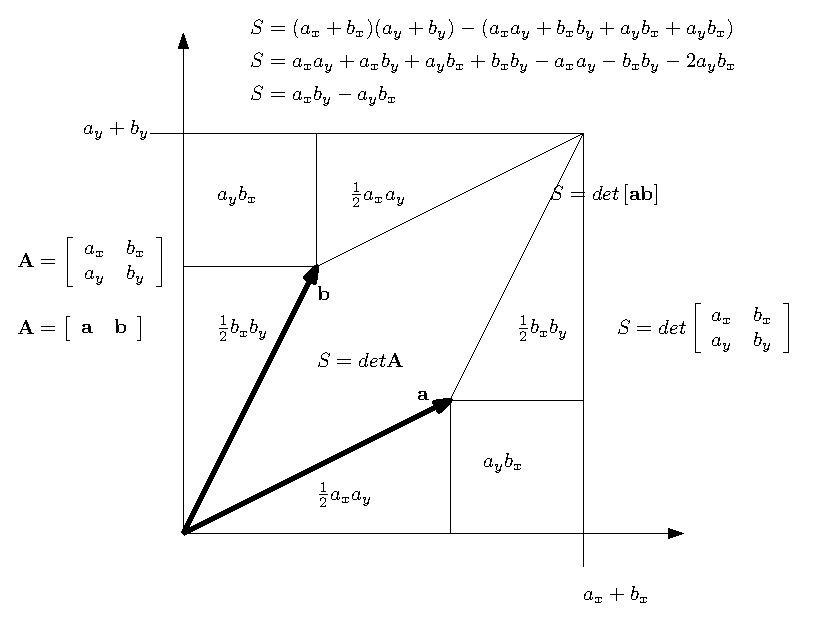
\includegraphics[width=7cm]{Math_matrix/determinantGeo.eps}
\end{figure}

\end{frame}
%%%%%%%%%%%%%%%%%%%%%%%%%%%%%%%%%%%%%%%%%%%%%%%%%%%%%%%%%


%%%%%%%%%%%%%%%%%%%%%%%%%%%%%%%%%%%%%%%%%%%%%%%%%%%%%%%%%
\begin{frame}{$3 \times 3$ 행렬의 행렬식 의미}

$\mathbf A \in \mathbb R^{3 \times 3}$는 세 개의 벡터 $\mathbf a, \mathbf b, \mathbf c$를 포함

$$
\mathbf A = \left [ \begin{array}{ccc}
a_1 & b_1 & c_1 \\
a_2 & b_2 & c_2 \\
a_3 & b_3 & c_3 
\end{array} \right ] =
\left [ \begin{array}{ccc}
\mathbf a & \mathbf b & \mathbf c
\end{array} \right ] 
$$

이 세 개의 벡터들이 만드는 평행육면체의 크기가 세 개의 벡터들로 구성된 행렬의 행렬식


\begin{figure}
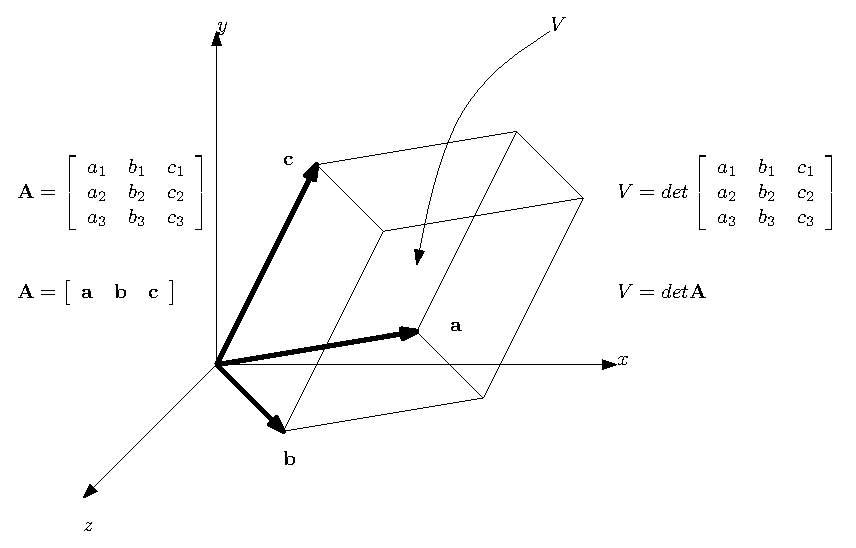
\includegraphics[width=7cm]{Math_matrix/determinantGeo3D.eps}
\end{figure}

\end{frame}
%%%%%%%%%%%%%%%%%%%%%%%%%%%%%%%%%%%%%%%%%%%%%%%%%%%%%%%%%


%%%%%%%%%%%%%%%%%%%%%%%%%%%%%%%%%%%%%%%%%%%%%%%%%%%%%%%%%
\begin{frame}{행렬과 행렬식의 기하적 의미}

\begin{figure}
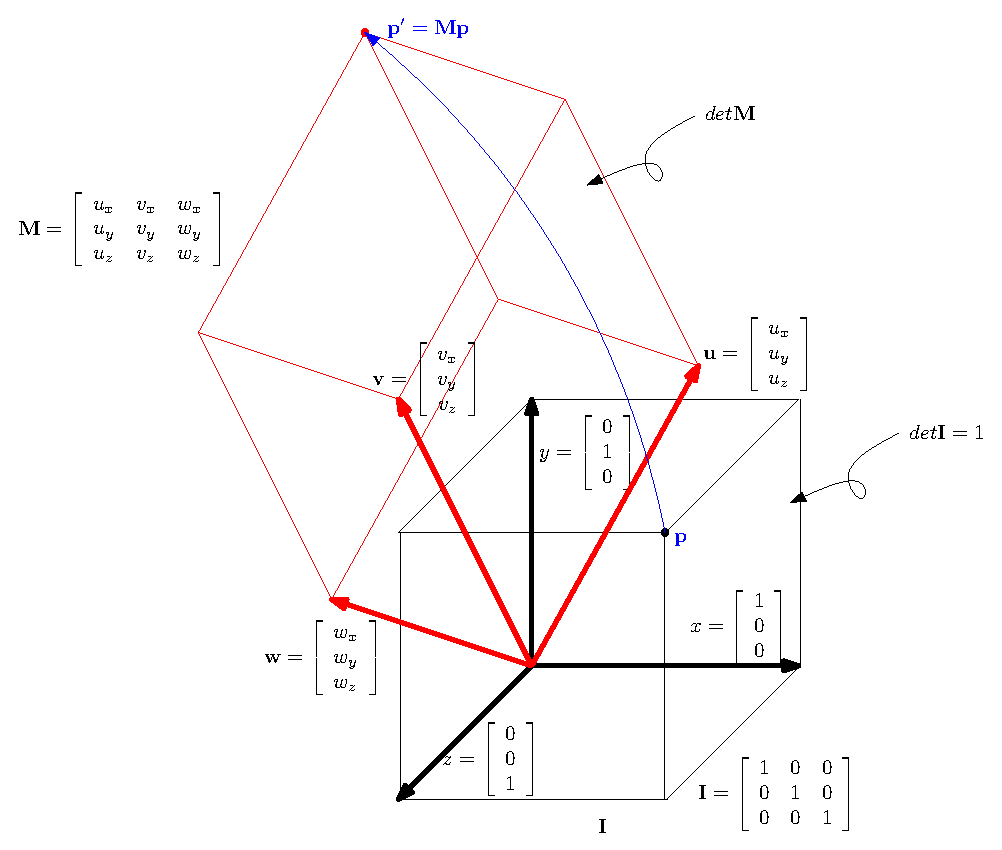
\includegraphics[width=8cm]{Math_matrix/matrixConcept.eps}
\end{figure}

\end{frame}
%%%%%%%%%%%%%%%%%%%%%%%%%%%%%%%%%%%%%%%%%%%%%%%%%%%%%%%%%

%%%%%%%%%%%%%%%%%%%%%%%%%%%%%%%%%%%%%%%%%%%%%%%%%%%%%%%%%
\begin{frame}{행렬식의 특성}

몇 가지 기억해 둘 행렬식의 특성은 다음과 같다.

$$|\mathbf A| = |\mathbf A^{\rm T}|$$

$$\mathbf A \in \mathbb R^{n \times n} \Rightarrow | k \mathbf A | = k^n |\mathbf A|$$

$$|\mathbf {AB}| = |\mathbf A| |\mathbf B|$$

\end{frame}
%%%%%%%%%%%%%%%%%%%%%%%%%%%%%%%%%%%%%%%%%%%%%%%%%%%%%%%%%

%%%%%%%%%%%%%%%%%%%%%%%%%%%%%%%%%%%%%%%%%%%%%%%%%%%%%%%%%
\begin{frame}{역행렬}


\begin{itemize}
\item 역행렬은 정방행렬에만 존재
\item $\mathbf A$의 역행렬이 존재한다면, 이 역행렬을 $\mathbf A^{-1}$로 표현
\item 역행렬 $\mathbf A^{-1}$은 다음과 같은 조건을 만족
	\begin{itemize}
	\item $\mathbf {AA}^{-1} = \mathbf I$
	\item $\mathbf A^{-1} \mathbf A = \mathbf I$
	\end{itemize}
\end{itemize}

\begin{itemize}
\item 역행렬이 존재하는 행렬을 가역행렬(invertible matrix)
\item 역행렬이 존재하지 않는 행렬은 특이행렬(singular matrix)
\end{itemize}

\begin{itemize}
\item 의사 역행렬(pseudo-inverse)
	\begin{itemize}
	\item  행렬 $\mathbf A$가 정방행렬이 아니고 $\mathbb R^{m \times n}$에 속한다고 하자. 다른 어떤 행렬 $\mathbf B$가 $\mathbb R^{n \times m}$에 속하면, 두 행렬의 곱 $\mathbf {AB}$는 $\mathbb R^{m \times m}$에 속하는 정방행렬이 된다. 만약 $\mathbf {AB} = \mathbf I \in \mathbb R^{n \times n}$이라면, $\mathbf B$를 $\mathbf A$의 의사 역행렬(pseudo-inverse)라고 한다.
	\end{itemize}
\end{itemize}
\end{frame}
%%%%%%%%%%%%%%%%%%%%%%%%%%%%%%%%%%%%%%%%%%%%%%%%%%%%%%%%%


%%%%%%%%%%%%%%%%%%%%%%%%%%%%%%%%%%%%%%%%%%%%%%%%%%%%%%%%%
\begin{frame}{역행렬의 계산}

\begin{itemize}
\item 역행렬의 계산은 수반행렬(adjoint matrix)를 이용하여 쉽게 정의
	\begin{itemize}
	\item 행렬 $\mathbf A$의 수반행렬: 여인자 $C_{ij}$를 성분으로 하는 행렬 $\mathbf C$의 전치(transpose)
	\end{itemize}
\end{itemize}


$$ adj \mathbf A = 
\left (
\begin{array}{cccc}
C_{11} & C_{21} & \cdots & C_{n1} \\
C_{12} & C_{22} & \cdots & C_{n2} \\
\vdots & \vdots & \ddots & \vdots \\
C_{1n} & C_{2n} & \cdots & C_{nn} \\
\end{array}
\right )
= \mathbf C^{\rm T}
$$
 
\begin{itemize}
\item 수반행렬을 행렬의 행렬식으로 나누면 역행렬이 된다.
\end{itemize}

$$\mathbf A^{-1} = \frac{adj \mathbf A}{|\mathbf A|} = 
\frac{1}{|\mathbf A|}
\left (
\begin{array}{cccc}
C_{11} & C_{21} & \cdots & C_{n1} \\
C_{21} & C_{22} & \cdots & C_{n2} \\
\vdots & \vdots & \ddots & \vdots \\
C_{n1} & C_{2n} & \cdots & C_{nn} \\
\end{array}
\right )
= \mathbf C^{\rm T}
$$

식은 간단하지만, 여인자를 구하는 재귀호출이 매우 많은 계산을 요구

\end{frame}
%%%%%%%%%%%%%%%%%%%%%%%%%%%%%%%%%%%%%%%%%%%%%%%%%%%%%%%%%


%%%%%%%%%%%%%%%%%%%%%%%%%%%%%%%%%%%%%%%%%%%%%%%%%%%%%%%%%
\begin{frame}{변환이란}

수학적 의미에서 변환(transformation)

\begin{itemize}
\item 어떤 집합 $S$를 다른 어떤 집합 $S$로 대응시키는 함수
\item 공간과 점, 그리고 벡터의 문제로 이해할 때, 변환이란 공간 상의 벡터나 점을 다른 벡터나 점으로 바꾸는 연산
\item 변환 행렬
	\begin{itemize}
	\item 어떤 벡터 $\mathbf a$가 $\mathbb R^{n}$에 속한다고 할 때, 이 벡터에 행렬 $\mathbf A \in \mathbb R^{n \times n}$을 곱하면 $\mathbf a$와 같은 차원의 벡터 $\mathbf b$를 얻는다.
	\item $\mathbf b = \mathbf A \mathbf a ~ (\mathbf a, \mathbf b \in \mathbb R^n , \mathbf A \in \mathbb R^{n \times n})$.
	\item 어떤 벡터를 동일한 차원의 다른 벡터로 옮기는 행렬 $\mathbf A \in \mathbb R^{n \times n}$을 변환행렬(transform matrix)라고 한다.
	\end{itemize}
\end{itemize}

\end{frame}
%%%%%%%%%%%%%%%%%%%%%%%%%%%%%%%%%%%%%%%%%%%%%%%%%%%%%%%%%

%%%%%%%%%%%%%%%%%%%%%%%%%%%%%%%%%%%%%%%%%%%%%%%%%%%%%%%%%
\begin{frame}{좌표계 - 직교 좌표계}

\begin{itemize}
\item 일반적으로 가장 익숙한 좌표계
\item 데카르트 좌표계(Cartesian coordinate system)
\end{itemize}

\begin{figure}
    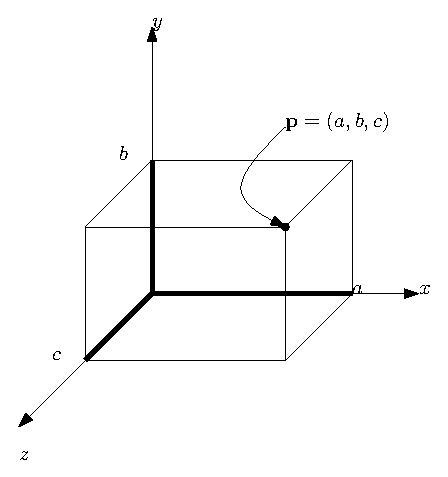
\includegraphics[width=6cm]{Math_transform/CartesianCoord.eps}
\end{figure}

\end{frame}
%%%%%%%%%%%%%%%%%%%%%%%%%%%%%%%%%%%%%%%%%%%%%%%%%%%%%%%%%

%%%%%%%%%%%%%%%%%%%%%%%%%%%%%%%%%%%%%%%%%%%%%%%%%%%%%%%%%
\begin{frame}{좌표계 - 원기둥 좌표계}

\begin{itemize}
\item $\mathbf p$는 이러한 높이 $h$와 반지름 $r$을 가진 원기둥의 윗쪽 원주에 놓임.
\item 원주에서 특정한 위치는 각도 $\theta$로 표현
\item 원기둥 좌표: $(r, \theta, h)$
\end{itemize}

\begin{figure}
    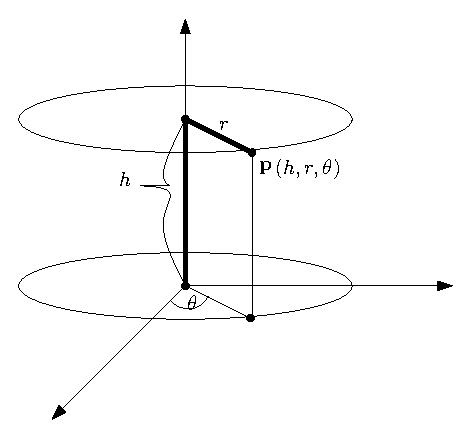
\includegraphics[width=6.5cm]{Math_transform/cylindricCoord.eps}
\end{figure}

\end{frame}
%%%%%%%%%%%%%%%%%%%%%%%%%%%%%%%%%%%%%%%%%%%%%%%%%%%%%%%%%

%%%%%%%%%%%%%%%%%%%%%%%%%%%%%%%%%%%%%%%%%%%%%%%%%%%%%%%%%
\begin{frame}{원기둥 좌표를 직교 좌표로 옮기기}

원기둥 좌표계의 좌표를 $\mathbf p_{cyl}$, 직교 좌표계의 좌표를 $\mathbf p_{cart}$으로 표현하면

$$(r, \theta, h)_{cyl} = ( r \cos \theta , r \sin \theta, h)_{cart}$$

\begin{figure}[h!]
  \centering
    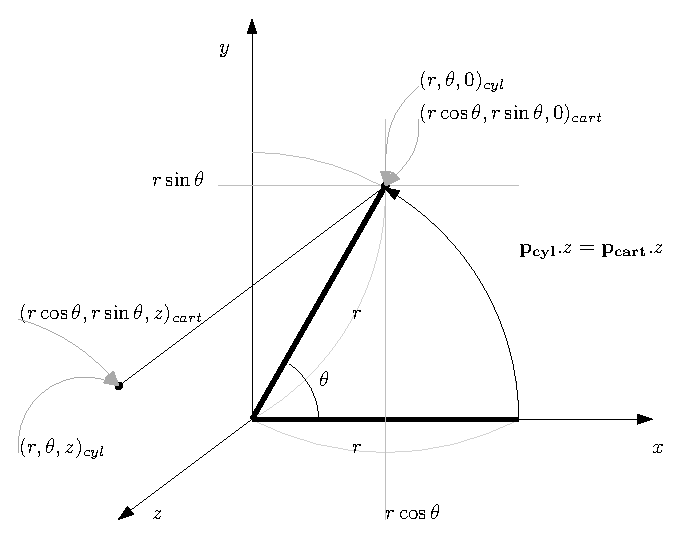
\includegraphics[width=6.5cm]{Math_transform/cyl2Cartesian.eps}
\end{figure}

\end{frame}
%%%%%%%%%%%%%%%%%%%%%%%%%%%%%%%%%%%%%%%%%%%%%%%%%%%%%%%%%


%%%%%%%%%%%%%%%%%%%%%%%%%%%%%%%%%%%%%%%%%%%%%%%%%%%%%%%%%
\begin{frame}{좌표계 - 구면 좌표계}

\begin{itemize}
\item $\mathbf p$를 지나며 중심이 원점인 구면의 반지름을 $r$
\item 반지름 $r$인 점 가운데  $x$ 축 위에 있는 점을 $\mathbf p_x$
\item $\mathbf p_x$을 $xy$ 평면 위에서 $\mathbf p$와 같은 경도선에 놓는 각도가 $\phi$
\item 이를 들어 올려 점 $\mathbf p$를 지나도록 하는 데에 필요한 각도를 $\theta$
\item 구면 좌표 $(r, \theta, \phi)$
\end{itemize}

\begin{figure}
    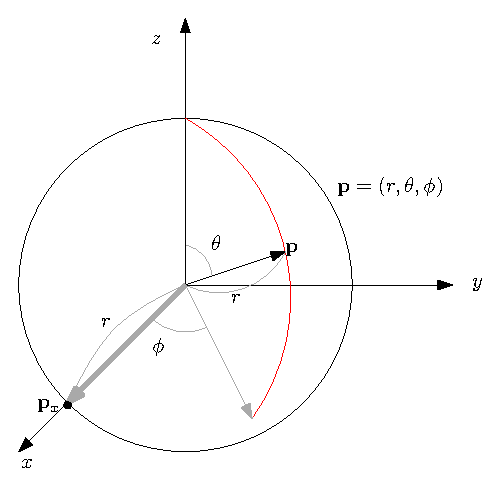
\includegraphics[width=5cm]{Math_transform/sphericalCoord.eps}
\end{figure}

\end{frame}
%%%%%%%%%%%%%%%%%%%%%%%%%%%%%%%%%%%%%%%%%%%%%%%%%%%%%%%%%

%%%%%%%%%%%%%%%%%%%%%%%%%%%%%%%%%%%%%%%%%%%%%%%%%%%%%%%%%
\begin{frame}{구면 좌표와 직교 좌표}

{\small
구면 좌표는 일반적으로 다음과 같은 제한을 갖는다.
$$r \geq 0$$
$$0 \leq \theta \leq \pi$$
$$0 \leq \phi \leq 2 \pi $$

직교 좌표계의 좌표 $(x,y,z)$를 구면 좌표계로 옮기기

\begin{eqnarray}
r &= \sqrt{x^2 + y^2 + z^2} \nonumber \\
\theta & = \arccos \left ( \frac{z}{\sqrt{x^2 + y^2 + z^2}} \right ) \nonumber \\
\phi &= \arctan \left ( \frac{y}{x} \right ) \nonumber
\end{eqnarray}

구면 좌표계의 좌표를 직교 좌표로 옮기기

\begin{eqnarray}
x &= r \sin \theta \cos \phi \nonumber \\
y & = r \sin \theta \sin \phi \nonumber \\
z & =r \cos \theta \nonumber
\end{eqnarray}
}

\end{frame}
%%%%%%%%%%%%%%%%%%%%%%%%%%%%%%%%%%%%%%%%%%%%%%%%%%%%%%%%%

%%%%%%%%%%%%%%%%%%%%%%%%%%%%%%%%%%%%%%%%%%%%%%%%%%%%%%%%%
\begin{frame}{무슨 좌표계를 사용할 것인가}

\begin{itemize}
\item 공간에 존재하는 점을 다룰 때에는 어떠한 좌표계를 사용해도 무방
\item 컴퓨터 그래픽스 분야에서 가장 많이 사용되는 좌표계는 직교 좌표계
\item 우리는 직교 좌표계에서 변환에 대해 다룰 예정
\item 직교 좌표계를 기본적인 좌표계로 삼고 변환과 관련된 행렬 연산을 살필 것
\end{itemize}

\end{frame}
%%%%%%%%%%%%%%%%%%%%%%%%%%%%%%%%%%%%%%%%%%%%%%%%%%%%%%%%%


%%%%%%%%%%%%%%%%%%%%%%%%%%%%%%%%%%%%%%%%%%%%%%%%%%%%%%%%%
\begin{frame}{어파인(affine) 변환}

{\small
게임을 구현하기 위한 3차원 그래픽스에서 흔히 사용되는 변환

\begin{itemize}
\item 이동변환(translation): 주어진 변위 벡터만큼 좌표를 동일하게 옮김
\item 회전변환(rotation): 2차원은 기준점, 3차원은 기준축을 중심으로 돌림
\item 크기변경(scaling): 각 축 방향으로 주어진 비율에 따라 좌표 값이 커지거나 줄어든다.
\end{itemize}

이러한 변환은 어파인 변환(affine transformation)의 일종
\begin{itemize}
\item 서로 연결되어 있음을 의미하는 라틴어 `affinis'에서 유래
\item 직선 위의 점들을 직선을 유지한 상태로 변환하는 변환
\item 직선 위에서의 점들 사이의 거리 비가 변환된 직선 위에서 그대로 유지
\item 직선은 직선으로, 평행선은 평행선으로 유지
\item 실시간 컴퓨터 그래픽스에서는 여러 가지 효율성의 이유로 어파인 변환을 사용
\end{itemize}
}

\end{frame}
%%%%%%%%%%%%%%%%%%%%%%%%%%%%%%%%%%%%%%%%%%%%%%%%%%%%%%%%%


%%%%%%%%%%%%%%%%%%%%%%%%%%%%%%%%%%%%%%%%%%%%%%%%%%%%%%%%%
\begin{frame}{이동 변환(translation)}

{\small
\begin{itemize}
\item 2차원: 좌표 $(x,y)$를 $x$ 축 방향으로 $a$, $y$ 축 방향으로 $b$ 만큼 옮기기
\item $(x', y') = (x,y) + (a,b) = (x+a, y+a)$
\end{itemize}

\begin{itemize}
\item 모든 차원에 대해
어떤 벡터 $\mathbf a$를 변위 벡터 $\mathbf d$를 이용하여 $\mathbf x'$로 옮기는 이동 변환을 다음과 같이 벡터 더하기로 정의할 수 있음
	\begin{itemize}
	\item $\mathbf a \in \mathbb R^n, \mathbf d \in \mathbb R^n$
	\item $\mathbf x' = \mathbf a + \mathbf d~~~~\mathbf x' \in \mathbb R^n$
	\end{itemize}
\end{itemize}


\begin{figure}
    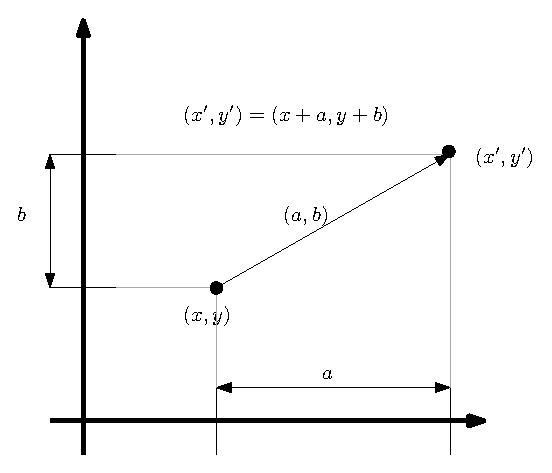
\includegraphics[width=5cm]{Math_transform/translation.eps}
\end{figure}
}

\end{frame}
%%%%%%%%%%%%%%%%%%%%%%%%%%%%%%%%%%%%%%%%%%%%%%%%%%%%%%%%%


%%%%%%%%%%%%%%%%%%%%%%%%%%%%%%%%%%%%%%%%%%%%%%%%%%%%%%%%%
\begin{frame}{2차원 회전 변환(rotation) - 문제}

{\small
\begin{itemize}
\item 2차원 회전의 중심: 피벗(pivot)
\item 기본적인 회전: 피벗이 원점인 경우
	\begin{itemize}
	\item $\mathbf p$를 원점을 중심으로 $\theta$ 만큼 회전하여 놓이는 지점 $\mathbf p'$를 구하는 문제
	\item 원래 좌표 $(p_x,p_y)$를 $\theta$ 만큼 회전하여 얻는 $(p'_x, p'_y)$를 얻는 문제
	\end{itemize}
\end{itemize}

\begin{figure}
    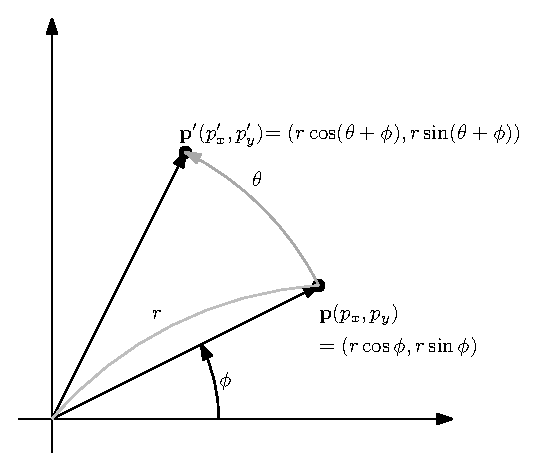
\includegraphics[width=6cm]{Math_transform/rotation.eps}
\end{figure}


}

\end{frame}
%%%%%%%%%%%%%%%%%%%%%%%%%%%%%%%%%%%%%%%%%%%%%%%%%%%%%%%%%


%%%%%%%%%%%%%%%%%%%%%%%%%%%%%%%%%%%%%%%%%%%%%%%%%%%%%%%%%
\begin{frame}{2차원 회전 변환(rotation) - 좌표값에 대한 이해}

\begin{figure}
    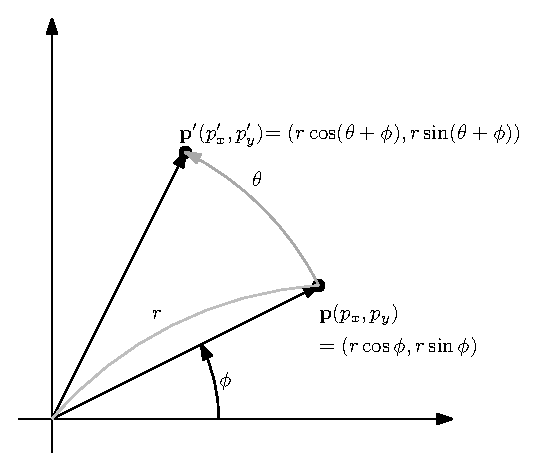
\includegraphics[width=5cm]{Math_transform/rotation.eps}
\end{figure}

\begin{itemize}
\item 원점에서 $(p_x,p_y)$로 선분: 선분 길이 $r$과 $x$축과 이루는 각도 $\phi$
\item $(p_x, p_y) = (r \cos \phi,  r \sin \phi)$
\item 이 좌표를 $\theta$만큼 회전하여 얻는 $(p'_x , p'_y)$
	\begin{itemize}
	\item $(p'_x, p'_y) =  ( r \cos (\theta+ \phi) , r \sin (\theta + \phi) )$
	\end{itemize}
\end{itemize}

\end{frame}
%%%%%%%%%%%%%%%%%%%%%%%%%%%%%%%%%%%%%%%%%%%%%%%%%%%%%%%%%


%%%%%%%%%%%%%%%%%%%%%%%%%%%%%%%%%%%%%%%%%%%%%%%%%%%%%%%%%
\begin{frame}{2차원 회전 변환(rotation) - 회전결과}

\begin{itemize}
\item $\phi$를 계산하지 않고 답을 얻어야 함
\item 참조할 공식
	\begin{itemize}
	\item $\cos (a+b) = \cos a \cos b - \sin a \sin b$
	\item $\sin (a+b) = \sin a \cos b + \cos a \sin b$
	\end{itemize}
\item 회전하여 얻는 좌표는 다음과 같이 표현
	\begin{itemize}
	\item $p'_x = (r \cos \phi) \cos \theta - (r \sin \phi )\sin \theta$
	\item $p'_y = (r \cos \phi) \sin \theta + (r \sin \phi )\cos \theta$
	\end{itemize}
\item 원래의 좌표 $(p_x , p_y )$를 이용하여 표현
	\begin{itemize}
	\item $p'_x = p_x \cos \theta - p_y \sin \theta$
	\item $p'_y = p_x \sin \theta + p_y \cos \theta$
	\end{itemize} 
\end{itemize}



\end{frame}
%%%%%%%%%%%%%%%%%%%%%%%%%%%%%%%%%%%%%%%%%%%%%%%%%%%%%%%%%

%%%%%%%%%%%%%%%%%%%%%%%%%%%%%%%%%%%%%%%%%%%%%%%%%%%%%%%%%
\begin{frame}{2차원 회전 변환(rotation) - 행렬표현}

이러한 변환은 다음과 같은 행렬과 벡터의 곱으로 표현할 수 있다.

\begin{eqnarray}
\left [
\begin{array}{c}
p'_x \\ p'_y
\end{array}
\right ] =
\left [
\begin{array}{cc}
\cos \theta & - \sin \theta \\
\sin \theta & \cos \theta
\end{array}
\right ]
\left [
\begin{array}{c}
p_x \\
p_y
\end{array}
\right ] \nonumber
\end{eqnarray}

2차원 공간에서 어떤 점 $\mathbf p$를 원점 기준으로 $\theta$만큼 회전시켜 $\mathbf p'$를 얻는 변환은 회전변환 행렬 $\mathbf R(\theta)$을
이용하여 $\mathbf p' = \mathbf R(\theta) \mathbf p$로 표현할 수 있다.

\begin{eqnarray}
\mathbf R(\theta) = \left [ 
\begin{array}{cc}
\cos \theta & - \sin \theta \\
\sin \theta & \cos \theta
\end{array}
\right ] \nonumber
\end{eqnarray} 

\end{frame}
%%%%%%%%%%%%%%%%%%%%%%%%%%%%%%%%%%%%%%%%%%%%%%%%%%%%%%%%%


%%%%%%%%%%%%%%%%%%%%%%%%%%%%%%%%%%%%%%%%%%%%%%%%%%%%%%%%%
\begin{frame}[fragile]{3차원 회전 - $z$ 축 회전}

\begin{itemize}
\item 2차원 회전을 그대로 3차원에 적용
	\begin{itemize}
	\item 3차원 좌표 $\mathbf p = (p_x, p_y, p_z)$을 $z$ 기준으로 회전
	\end{itemize}
\item 이 변환은 2차원 변환에 $z$ 성분만 추가
	\begin{itemize}
	\item $z$ 축 성분은 그대로 유지된다. ($p'_z = p_z)$
	\item $p_x, p_y$의 값은 2차원 회전과 동일하게 변환된다.
	\end{itemize}
\end{itemize}

\begin{eqnarray}
\begin{array}{clrrr} 
p'_x  & = &\cos \theta \cdot p_x &- \sin \theta \cdot p_y &+ 0 \cdot p_z \\
p'_y  & = &\sin \theta \cdot p_x &+ \cos \theta \cdot p_y &+ 0 \cdot p_z \\
p'_z  & = & 0 \cdot p_x &+ 0 \cdot p_y &+ 1 \cdot p_z
\end{array} \nonumber
\end{eqnarray}

이것은 다음과 같은 행렬 표현으로 다시 쓸 수 있다.

\begin{eqnarray}
\left [ \begin{array}{c} p'_x \\ p'_y \\ p'_z  \end{array} \right ] 
=
\left [ \begin{array}{rrr}
\cos \theta &- \sin \theta  & 0  \\
\sin \theta & \cos \theta  & 0 \\
0 & 0  & 1 
\end{array} \right ]
\left [ \begin{array}{c} p_x \\ p_y \\ p_z \end{array} \right ]  \nonumber
\end{eqnarray}


\end{frame}
%%%%%%%%%%%%%%%%%%%%%%%%%%%%%%%%%%%%%%%%%%%%%%%%%%%%%%%%%


%%%%%%%%%%%%%%%%%%%%%%%%%%%%%%%%%%%%%%%%%%%%%%%%%%%%%%%%%
\begin{frame}{3차원 회전 - $y$ 축 회전 (1/2)}

\begin{figure}
    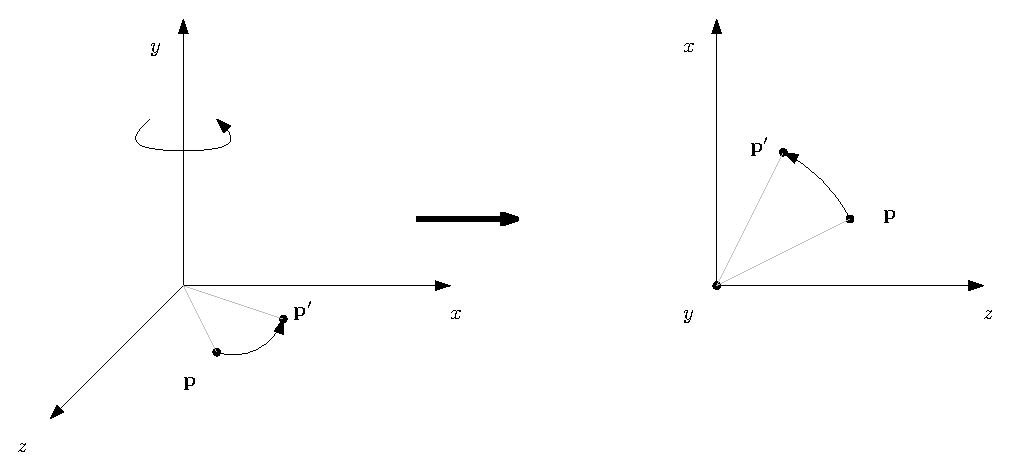
\includegraphics[width=10cm]{Math_transform/yAxisRotation.eps}
\end{figure}

\begin{itemize}
\item $z$ 축은 2차원 회전의 $x$축에 대응
\item $x$ 축은 2차원 회전의 $y$축에 대응
\end{itemize}

\begin{eqnarray}
\begin{array}{clrrr}
p'_z  & = &\cos \theta \cdot p_z &- \sin \theta \cdot p_x &+ 0 \cdot p_y \\
p'_x  & = &\sin \theta \cdot p_z &+ \cos \theta \cdot p_x &+ 0 \cdot p_y \\
p'_y  & = & 0 \cdot p_z &+ 0 \cdot p_x &+ 1 \cdot p_y
\end{array} \nonumber
\end{eqnarray}


\end{frame}
%%%%%%%%%%%%%%%%%%%%%%%%%%%%%%%%%%%%%%%%%%%%%%%%%%%%%%%%%


%%%%%%%%%%%%%%%%%%%%%%%%%%%%%%%%%%%%%%%%%%%%%%%%%%%%%%%%%
\begin{frame}{3차원 회전 - $y$ 축 회전 (1/2)}

순서를 재배열하면 다음과 같은 식을 얻는다.

\begin{eqnarray}
\begin{array}{clrrr}
p'_x  & = & \cos \theta \cdot p_x &+ 0 \cdot p_y &+ \sin \theta \cdot p_z  \\
p'_y  & =  &0 \cdot p_x &+ 1 \cdot p_y & 0 \cdot p_z \\
p'_z  & = &-\sin \theta \cdot p_x &+ 0 \cdot p_y  & + \cos \theta \cdot p_z 
\end{array} \nonumber
\end{eqnarray}

이것도 역시 행렬 표현으로 다시 쓸 수 있다.

\begin{eqnarray}
\left [ \begin{array}{c} p'_x \\ p'_y \\ p'_z  \end{array} \right ] 
=
\left [ \begin{array}{rrr}
\cos \theta & 0 &  \sin \theta  \\
0 & 1 & 0 \\
- \sin \theta & 0 & \cos \theta
\end{array} \right ]
\left [ \begin{array}{c} p_x \\ p_y \\ p_z \end{array} \right ]  \nonumber
\end{eqnarray}


\end{frame}
%%%%%%%%%%%%%%%%%%%%%%%%%%%%%%%%%%%%%%%%%%%%%%%%%%%%%%%%%

%%%%%%%%%%%%%%%%%%%%%%%%%%%%%%%%%%%%%%%%%%%%%%%%%%%%%%%%%
\begin{frame}{3차원 회전 - $x$ 축 회전 (1/2)}

\begin{itemize}
\item 2차원 회전에서 $x$, $y$의 역할에 $y$와 $z$ 축이 각각 대응
\end{itemize}

\begin{figure}
    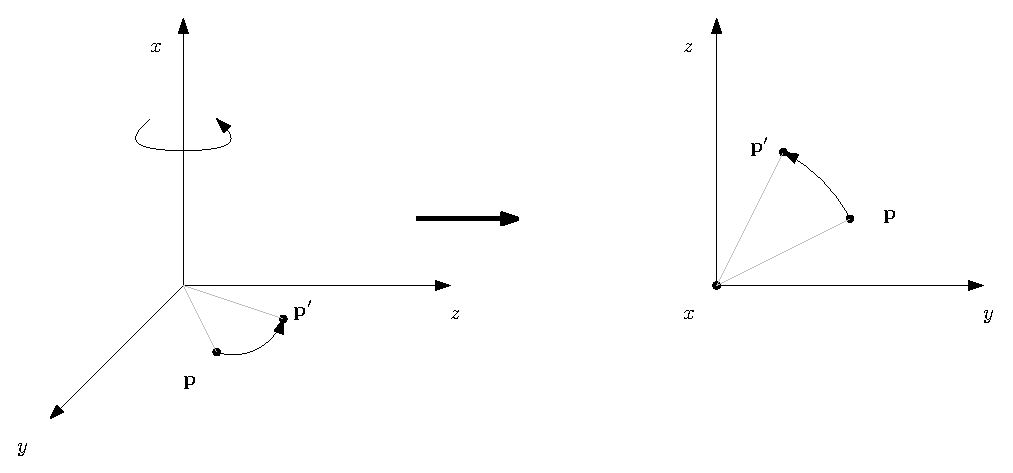
\includegraphics[width=10cm]{Math_transform/xAxisRotation.eps}
\end{figure}

\begin{eqnarray}
\begin{array}{clrrr}
p'_y  & = &\cos \theta \cdot p_y &- \sin \theta \cdot p_z &+ 0 \cdot p_x \\
p'_z  & = &\sin \theta \cdot p_y &+ \cos \theta \cdot p_z &+ 0 \cdot p_x \\
p'_x  & = & 0 \cdot p_y &+ 0 \cdot p_z &+ 1 \cdot p_x
\end{array} \nonumber
\end{eqnarray}


\end{frame}
%%%%%%%%%%%%%%%%%%%%%%%%%%%%%%%%%%%%%%%%%%%%%%%%%%%%%%%%%

%%%%%%%%%%%%%%%%%%%%%%%%%%%%%%%%%%%%%%%%%%%%%%%%%%%%%%%%%
\begin{frame}{3차원 회전 - $x$ 축 회전 (2/2)}

행렬과 벡터의 곱으로 표현하면 다음과 같다.

\begin{eqnarray}
\left [ \begin{array}{c} p'_x \\ p'_y \\ p'_z  \end{array} \right ] 
=
\left [ \begin{array}{rrr}
1 & 0 & 0 \\
0 & \cos \theta & - \sin \theta \\
0 & \sin \theta & \cos \theta
\end{array} \right ]
\left [ \begin{array}{c} p_x \\ p_y \\ p_z \end{array} \right ]  \nonumber
\end{eqnarray}

\end{frame}
%%%%%%%%%%%%%%%%%%%%%%%%%%%%%%%%%%%%%%%%%%%%%%%%%%%%%%%%%

%%%%%%%%%%%%%%%%%%%%%%%%%%%%%%%%%%%%%%%%%%%%%%%%%%%%%%%%%
\begin{frame}{회전 행렬의 역행렬}

\begin{itemize}
\item 회전행렬은 특별한 특징을 지님 (2차원 회전행렬을 보자)
	\begin{itemize}
	\item 첫 열 벡터는 길이는 $\sqrt{ \cos^2 \theta + \sin^2 \theta}$이므로 1
	\item 두 번째 열의 길이 역시 $\sqrt{ \sin^2 \theta + \cos^2 \theta}$로 1
	\item 즉 두 벡터 모두 단위 벡터 (정규)
	\item 이 두 벡터를 서로 내적하면 $\cos \theta ( - \sin \theta) + \sin \theta  \cos \theta $로 0
	\item 두 벡터가 서로 수직 (직교)
	\end{itemize}
\item 모든 벡터는 단위 벡터이고 서로 직교 = 정규직교(orthonormal)
\item 정규직교 행렬의 역행렬은 그 행렬의 전치(transpose)와 같음
\item 3차원 회전행렬들도 정규직교임을 쉽게 확인 가능
\end{itemize}

$${{\mathbf R}_x}^{-1}(\theta) = {{\mathbf R}_x}^{\rm T}(\theta)$$
$${{\mathbf R}_y}^{-1}(\theta) = {{\mathbf R}_y}^{\rm T}(\theta)$$
$${{\mathbf R}_z}^{-1}(\theta) = {{\mathbf R}_z}^{\rm T}(\theta)$$

\end{frame}
%%%%%%%%%%%%%%%%%%%%%%%%%%%%%%%%%%%%%%%%%%%%%%%%%%%%%%%%%

%%%%%%%%%%%%%%%%%%%%%%%%%%%%%%%%%%%%%%%%%%%%%%%%%%%%%%%%%
\begin{frame}{임의의 축에 대한 회전}

\begin{itemize}
\item 임의의 회전축을 기준으로  $\theta$만큼 회전하는 변환은 다음과 같은 절차를 따라 구현할 수 있다.

	\begin{enumerate}
	\item 회전축이 원점을 지나도록 이동변환 $\mathbf T$를 적용한다.
	\item 원점을 지나는 회전축이 $xz$ 평면에 놓이도록 $z$축 회전 $\mathbf R_1$ 적용
	\item 이 회전축이 $z$축과 동일한 방향이 되도록 $y$축 회전 $\mathbf R_2$를 적용한다.
	\item $z$축을 기준으로 $\theta$만큼 회전하도록 $\mathbf R_z(\theta)$를 적용한다.
	\item ${\mathbf R_2}^{-1}$, 즉 ${\mathbf R_2}^{\rm T}$를 적용한다.
	\item ${\mathbf R_1}^{-1}$, 즉 ${\mathbf R_1}^{\rm T}$를 적용한다.
	\item $\mathbf T^{-1}$, 즉 $- \mathbf T$를 적용한다.
	\end{enumerate}

\item 벡터 더하기(이동변환)와 행렬 곱하기(회전)가 혼재
\item 동차좌표계(homogeneous coordinate)을 이용
	\begin{itemize}
	\item 이동 변환과 회전 변환 모두 $4 \times 4$ 행렬
	\item 위의 절차를 모두 누적한 하나의 행렬로 표현 가능
	\end{itemize}
\item $\mathbf R_{pivot}(\theta) = - \mathbf T {\mathbf R_1}^{\rm T} {\mathbf R_2}^{\rm T}  \mathbf R_z(\theta) \mathbf R_2  \mathbf R_1 \mathbf T $
\end{itemize}


\end{frame}
%%%%%%%%%%%%%%%%%%%%%%%%%%%%%%%%%%%%%%%%%%%%%%%%%%%%%%%%%


%%%%%%%%%%%%%%%%%%%%%%%%%%%%%%%%%%%%%%%%%%%%%%%%%%%%%%%%%
\begin{frame}{동차좌표계(homogeneous coordinate)}

\begin{itemize}
\item 사영기하학(射影幾何學, projective geometry)에서 사용되는 좌표계
\item $n$ 차원의 사영공간을 $n+1$의 좌표로 표현
\item 그래픽 API나 라이브러리들은 동차좌표계를 표준적인 좌표계로 채용
	\begin{itemize}
	\item 3차원 그래픽스에서 정의된 3차원 가상 공간 객체의 2차원 투영 이미지를 얻는 일과 유관
	\item 3차원 공간의 어파인(affine) 변환들을 모두 $4 \times 4$의 행렬로 표현
	\end{itemize}
\item 3차원 공간의 좌표를 표현하는 벡터 $[x,y,z]^{\rm T}$는 동차좌표계에서 $[x,y,z,1]^{\rm T}$로 표현할 수 있음
\item 보다 일반적인 형태는 마지막 숫자를 1이 아닌 다른 값게 하는 것
\item 2차원: $[x,y,w]^{\rm T}$, 3차원: $[x,y,z,w]^{\rm T}$
\end{itemize}

\end{frame}
%%%%%%%%%%%%%%%%%%%%%%%%%%%%%%%%%%%%%%%%%%%%%%%%%%%%%%%%%


%%%%%%%%%%%%%%%%%%%%%%%%%%%%%%%%%%%%%%%%%%%%%%%%%%%%%%%%%
\begin{frame}{동차좌표계의 시각적 이해 (1/2)}

동차좌표계 이해를 위해 Ammeraal이 사용한 그림

\begin{figure}
    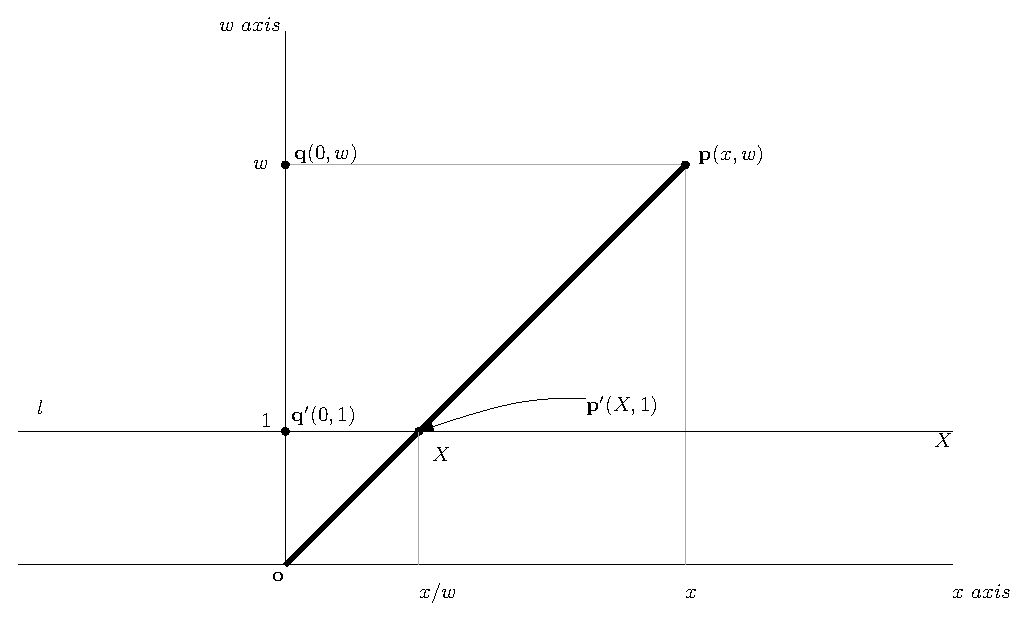
\includegraphics[width=12cm]{Math_transform/homogeneousConcept.eps}
\end{figure}

\end{frame}
%%%%%%%%%%%%%%%%%%%%%%%%%%%%%%%%%%%%%%%%%%%%%%%%%%%%%%%%%



%%%%%%%%%%%%%%%%%%%%%%%%%%%%%%%%%%%%%%%%%%%%%%%%%%%%%%%%%
\begin{frame}{동차좌표계의 시각적 이해 (2/2)}

\begin{itemize}
\item 두개의 축: $x$ 축이고, 다른 하나는 $w$ 축
	\begin{itemize}
	\item 동차 좌표계에서 마지막 원소 $w$를 제외한 모든 성분은 이 $x$ 축 값
	\item 마지막 원소는 이 $w$ 축 값
	\end{itemize}
\item $x$축 위에 있지 않는 점 $\mathbf p$는 중심 사영(central projection) $\mathbf p'$를 가짐
	\begin{itemize}
	\item $w=1$의 직선 $l$과 원점 $\mathbf o$에서 $\mathbf p$를 연결한 직선의 교차점
	\item 이때 원점은 사영중심(center of projection)
	\end{itemize}
\item $w$ 축과 $x$축을 모두 포함한 차원의 공간을 이보다 한 차원 낮은 $x$축 공간으로 떨어뜨리는 것
\item 선분 $\overline{\mathbf o \mathbf p}$를 지나는 직선 위의 모든 점들이 이 $\mathbf p'$로 사영
\item $(x,w)$에 해당하는 $\mathbf p'(X,1)$ 구하기
	\begin{itemize}
	\item 닮은 삼각형 $\mathbf{opq}$와 $\mathbf{op'q'}$
	\item 등비 관계를 이용하여 구한다
	\item $X = \frac{X}{1} = \frac{|\mathbf{p'q'}|}{|\mathbf{oq'}|}$
	\end{itemize}
\item 이 식은 다음과 같이 바뀐다.
\item $X = \frac{X}{1} = \frac{|\mathbf{oq'}|}{|\mathbf{p'q'}|} = \frac{|\mathbf{oq}|}{|\mathbf{pq}|} = \frac{x}{w} $
\end{itemize}



\end{frame}
%%%%%%%%%%%%%%%%%%%%%%%%%%%%%%%%%%%%%%%%%%%%%%%%%%%%%%%%%

%%%%%%%%%%%%%%%%%%%%%%%%%%%%%%%%%%%%%%%%%%%%%%%%%%%%%%%%%
\begin{frame}{동차좌표계와 데카르트 좌표계의 관계}

\begin{block}{$w$ 좌표의 의미}
사영기하에서 $\mathbf {op}$를 지나는 직선 위의 모든 점들은 $(x,w)$ 형태의 좌표로 표현할 수 있고,
이 모든 점들은 $w=1$인 평면으로 중심사영을 수행했을 때, $w$ 좌표는 무의미해지면서 $(x/w)$의 좌표로 바뀌게 된다.
즉, 3차원 공간의 좌표를 표현하기 위해 동차좌표계를 사용한다면 $[x,y,z,w]^{\rm T}$의 형태가 되며,
이것은 위의 그림에서 $w$ 축을 포함한 공간이 된다. 이를 3차원 데카르트 좌표로 바꾸는 것은 
중심사영이 이루어지는 $w=1$ 평면으로 옮겨 놓는 것이고 이때의 좌표는 $[x/w,y/w,z/w]^{\rm T}$가 되는 것이다.
그리고 3차원 공간의 측면에서 보면, $\mathbf {op}$를 지나는 직선 위의 모든 점들이 동일한 점으로 간주되는 것이다.
\end{block}

\end{frame}
%%%%%%%%%%%%%%%%%%%%%%%%%%%%%%%%%%%%%%%%%%%%%%%%%%%%%%%%%


%%%%%%%%%%%%%%%%%%%%%%%%%%%%%%%%%%%%%%%%%%%%%%%%%%%%%%%%%
\begin{frame}{동차 좌표계 사용의 이점(利點)}

\begin{itemize}
\item 3차원 좌표 $[x,y,z]^{\rm T}$를 동차좌표계 좌표로 바꾸는 간단한 방법은 $w=1$ 평면에서의 좌표인 $[x,y,z,1]^{\rm T}$
\item 동차좌표계를 쓰면 좋은 점
	\begin{itemize}
	\item 좌표와 벡터의 구분이 가능
	\item $[x,y,z]^{\rm T}$가 3차원 좌표라면 이 좌표로 표현되는 지점은 3차원 공간내 유일
	\item 벡터로 해석된다면 그것은 수 많은 동등 벡터를 표현하게 되며, 공간 내의 특별한 지점을 가리키지 않음
	\item 이 둘은 분명히 다르지만 단순한 좌표 표현 방식으로는 구분이 불가능
	\end{itemize}
\item 동차좌표계에서 좌표와 벡터의 구분
	\begin{itemize}
	\item 좌표는 $w \neq 0$인 $[x,y,z,w]^{\rm T}$
	\item 벡터는 $w = 0$인 $[x,y,z,0]^{\rm T}$
	\item $[x,y,z,0]^{\rm T}$는 위치를 가진 좌표 $[x,y,z]^{\rm T}$가 아니라 위치가 없는 벡터 $[x,y,z]^{\rm T}$
	\end{itemize}
\item 또다른 잇점
	\begin{itemize}
	\item 이동변환와 회전변환을 모두 같은 차원의 행렬로 표현
	\end{itemize}
\end{itemize}


\end{frame}
%%%%%%%%%%%%%%%%%%%%%%%%%%%%%%%%%%%%%%%%%%%%%%%%%%%%%%%%%

%%%%%%%%%%%%%%%%%%%%%%%%%%%%%%%%%%%%%%%%%%%%%%%%%%%%%%%%%
\begin{frame}{동차 좌표계에서 이동 변환}

동차좌표계에서의 이동

\begin{eqnarray}
\left [
\begin{array}{c}
x' \\y' \\ z' \\ 1
\end{array}
\right ]
=
\left [
\begin{array}{c}
x \\ y \\ z \\ 1
\end{array}
\right ]
+
\left [
\begin{array}{c}
d_x \\ d_y \\ d_z \\ 0
\end{array}
\right ]
=
\left [
\begin{array}{c}
x+d_x \\ y+d_y \\ z+d_z \\ 1
\end{array}
\right ] \nonumber
\end{eqnarray}


행렬 표현


\begin{eqnarray}
\left [
\begin{array}{c}
x' \\y' \\ z' \\ 1
\end{array}
\right ]
=
\left [
\begin{array}{cccc}
1 & 0 & 0 & d_x \\
0 & 1 & 0 & d_y \\
0 & 0 & 1 & d_z \\
0 & 0 & 0 & 1 \\
\end{array}
\right ]
\left [
\begin{array}{c}
x \\ y \\ z \\ 1
\end{array}
\right ]
=
\left [
\begin{array}{c}
x+d_x \\ y+d_y \\ z+d_z \\ 1
\end{array}
\right ] \nonumber
\end{eqnarray}


\end{frame}
%%%%%%%%%%%%%%%%%%%%%%%%%%%%%%%%%%%%%%%%%%%%%%%%%%%%%%%%%

%%%%%%%%%%%%%%%%%%%%%%%%%%%%%%%%%%%%%%%%%%%%%%%%%%%%%%%%%
\begin{frame}{이동 변환 행렬의 역행렬}

이제 이동변환을 행렬로 표현할 수 있게 되었다. 변위 벡터 $\mathbf d(d_x,d_y,d_z)$ 만큼의 이동을 수행하는 변환행렬을 $\mathbf T_{\mathbf d}$라고 하면
이동 변환은 다음과 같이 표현할 수 있다.

$$\mathbf p' = \mathbf T_{\mathbf d} \mathbf p, ~~~\mathbf T_{\mathbf d} \in \mathbb R^{4 \times 4}$$

이동변환 행렬 $\mathbf T_{\mathbf d}$의 역행렬은 어떻게 될까? 역행렬은 이 행렬이 일으킨 변환을 원래대로 되돌려 놓는 것이므로 
$\mathbf T_{- \mathbf d}$가 됨을 알 수 있다.

$$
\left [
\begin{array}{cccc}
1 & 0 & 0 & d_x \\
0 & 1 & 0 & d_y \\
0 & 0 & 1 & d_z \\
0 & 0 & 0 & 1 \\
\end{array}
\right ]^{-1}
= 
\left [
\begin{array}{cccc}
1 & 0 & 0 & -d_x \\
0 & 1 & 0 & -d_y \\
0 & 0 & 1 & -d_z \\
0 & 0 & 0 & 1 \\
\end{array}
\right ]
$$



\end{frame}
%%%%%%%%%%%%%%%%%%%%%%%%%%%%%%%%%%%%%%%%%%%%%%%%%%%%%%%%%


%%%%%%%%%%%%%%%%%%%%%%%%%%%%%%%%%%%%%%%%%%%%%%%%%%%%%%%%%
\begin{frame}{동차좌표계에서의 회전 행렬}

\begin{itemize}
\item 3차원 공간에서 정의되었던 회전 변환을 $\mathbf R_{33}$
\item $\mathbb R^{4 \times 4}$에 속하는 동차좌표계 회전 행렬은 $\mathbf R_{44}$
\item 원소가 모두 0인 3차원 열벡터를 $\mathbf O_3^{col}$, 행벡터를 $\mathbf O_3^{row}$
\end{itemize}

$$\mathbf R_{44} = 
\left [
\begin{array}{cc}
\mathbf R_{33} & \mathbf O_3^{col} \\
\mathbf O_3^{row} & 1
\end{array}
\right ]
$$

$
\mathbf R_{44}^x =
\left [
\begin{array}{cccc}
 1 & 0 & 0 & 0 \\
 0 & \cos \theta & -\sin \theta &  0\\
 0  & \sin \theta & cos \theta & 0 \\
 0 & 0 & 0 & 1 \\
\end{array}
\right ]
$
$
\mathbf R_{44}^y =
\left [
\begin{array}{cccc}
 \cos \theta & 0 & \sin \theta & 0 \\
 0 & 1 & 0 & 0 \\
- \sin \theta & 0  & \cos \theta & 0 \\
 0 & 0 & 0 & 1\\
\end{array}
\right ]
$

$$
\mathbf R_{44}^z =
\left [
\begin{array}{cccc}
 \cos \theta & - \sin \theta & 0 & 0 \\
 \sin \theta  & \cos \theta & 0 & 0 \\
 0 & 0 & 1 & 0 \\
 0 & 0 & 0 & 1\\
\end{array}
\right ]
$$



\end{frame}
%%%%%%%%%%%%%%%%%%%%%%%%%%%%%%%%%%%%%%%%%%%%%%%%%%%%%%%%%

%%%%%%%%%%%%%%%%%%%%%%%%%%%%%%%%%%%%%%%%%%%%%%%%%%%%%%%%%
\begin{frame}{복합변환}


좌표를 $\mathbf R_{44}$를 이용하여 회전하고, 이를 $\mathbf T_{\mathbf d}$ 만큼 이동하는 변환
\begin{eqnarray}
\mathbf p' = \mathbf T_{\mathbf d} \mathbf R_{44}  \mathbf p \nonumber
\end{eqnarray}

두 변환을 모두 수행하는 하나의 행렬 구할 수 있음 

\begin{eqnarray}
\mathbf p' & = &
\left [
\begin{array}{cc}
\mathbf I_{33} & \mathbf d \\
\mathbf O_3^{row} & 1
\end{array}
\right ]
\left [
\begin{array}{cc}
\mathbf R_{33} & \mathbf O_3^{col} \\
\mathbf O_3^{row} & 1
\end{array}
\right ]
\mathbf p \nonumber \\
& = &
\Large{
\left [
\begin{array}{cc}
\mathbf R_{33} & \mathbf d \\
\mathbf O_3^{row} & 1
\end{array}
\right ]
\mathbf p} \nonumber
\end{eqnarray}

\begin{itemize}
\item 행렬의 역행렬은?
\end{itemize}

\begin{eqnarray}
\left [
\begin{array}{cc}
\mathbf R_{33}^{\rm T} & \mathbf O_3^{col} \\
\mathbf O_3^{row} & 1
\end{array}
\right ]
\left [
\begin{array}{cc}
\mathbf I_{33} & - \mathbf d \\
\mathbf O_3^{row} & 1
\end{array}
\right ]
= 
\Large{
\left [
\begin{array}{cc}
\mathbf R_{33}^{\rm T} & - \mathbf R_{33}^{\rm T} \mathbf d \\
\mathbf O_3^{row} & 1
\end{array}
\right ]
} \nonumber
\end{eqnarray}

\end{frame}
%%%%%%%%%%%%%%%%%%%%%%%%%%%%%%%%%%%%%%%%%%%%%%%%%%%%%%%%%


%%%%%%%%%%%%%%%%%%%%%%%%%%%%%%%%%%%%%%%%%%%%%%%%%%%%%%%%%
\begin{frame}{복합변환}


좌표를 $\mathbf R_{44}$를 이용하여 회전하고, 이를 $\mathbf T_{\mathbf d}$ 만큼 이동하는 변환
\begin{eqnarray}
\mathbf p' = \mathbf T_{\mathbf d} \mathbf R_{44}  \mathbf p \nonumber
\end{eqnarray}

두 변환을 모두 수행하는 하나의 행렬 구할 수 있음 

\begin{eqnarray}
\mathbf p' & = &
\left [
\begin{array}{cc}
\mathbf I_{33} & \mathbf d \\
\mathbf O_3^{row} & 1
\end{array}
\right ]
\left [
\begin{array}{cc}
\mathbf R_{33} & \mathbf O_3^{col} \\
\mathbf O_3^{row} & 1
\end{array}
\right ]
\mathbf p \nonumber \\
& = &
\Large{
\left [
\begin{array}{cc}
\mathbf R_{33} & \mathbf d \\
\mathbf O_3^{row} & 1
\end{array}
\right ]
\mathbf p} \nonumber
\end{eqnarray}

\begin{itemize}
\item 행렬의 역행렬은?
\end{itemize}

\begin{eqnarray}
\left [
\begin{array}{cc}
\mathbf R_{33}^{\rm T} & \mathbf O_3^{col} \\
\mathbf O_3^{row} & 1
\end{array}
\right ]
\left [
\begin{array}{cc}
\mathbf I_{33} & - \mathbf d \\
\mathbf O_3^{row} & 1
\end{array}
\right ]
= 
\Large{
\left [
\begin{array}{cc}
\mathbf R_{33}^{\rm T} & - \mathbf R_{33}^{\rm T} \mathbf d \\
\mathbf O_3^{row} & 1
\end{array}
\right ]
} \nonumber
\end{eqnarray}

\end{frame}
%%%%%%%%%%%%%%%%%%%%%%%%%%%%%%%%%%%%%%%%%%%%%%%%%%%%%%%%%

%%%%%%%%%%%%%%%%%%%%%%%%%%%%%%%%%%%%%%%%%%%%%%%%%%%%%%%%%
\begin{frame}{좌표계의 변환}


\begin{itemize}
\item 어떤 점이 좌표계 $A$에 의해 $\mathbf p_A$라 표현된다고 가정
\item 다른 좌표계 $B$의 입장에서 보면 다른 좌표 $\mathbf p_B$
\item 이렇게 좌표계가 달라질 때 바뀐 좌표계에 따라 새로운 좌표를 계산하는 일은 그래픽스에서 매우 빈번히 나타나는 작업
	\begin{itemize}
	\item 가상 공간 내의 모든 객체의 위치를 하나의 기준으로 정의하는 데에 필요한 전역좌표계(global coordinate system)과 개별 객체 내에 정의된 지역좌표계(local coordinate system)
	\end{itemize}
\end{itemize}

\end{frame}
%%%%%%%%%%%%%%%%%%%%%%%%%%%%%%%%%%%%%%%%%%%%%%%%%%%%%%%%%

%%%%%%%%%%%%%%%%%%%%%%%%%%%%%%%%%%%%%%%%%%%%%%%%%%%%%%%%%
\begin{frame}[fragile]{좌표계의 이동}


$\mathbf p_A = \mathbf p_B + \mathbf d$
\begin{figure}
    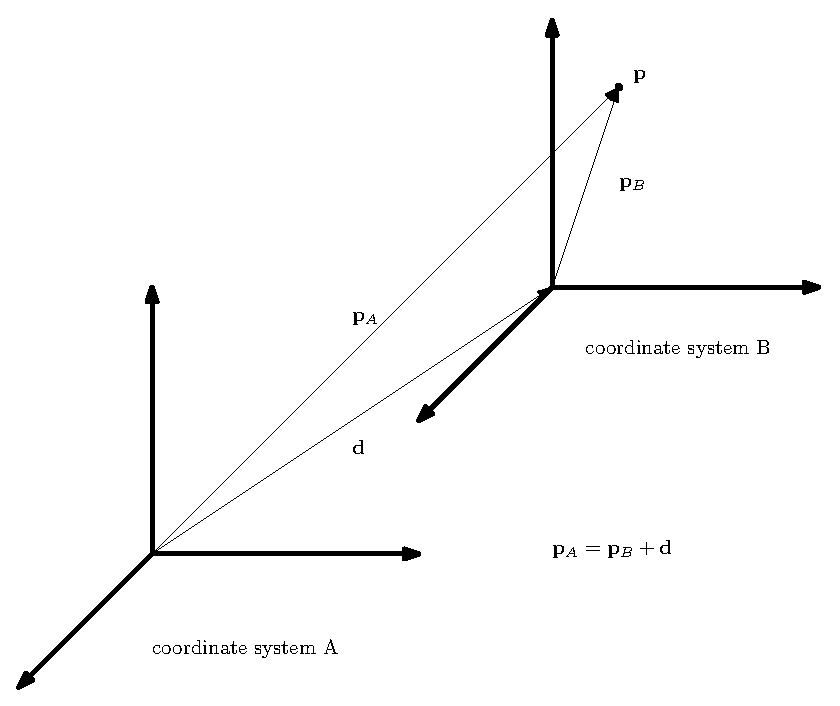
\includegraphics[width=6cm]{Math_transform/coordinateTranslate.eps}
\end{figure}

\begin{tabular}{lcc}
$
\mathbf T_{\mathbf d} = \left [
\begin{array}{cccc}
1 & 0 & 0 & d_x \\
0 & 1 & 0 & d_y \\
0 & 0 & 1 & d_z \\
0 & 0 & 0 & 1 \\
\end{array}
\right ],
$ &
$\mathbf p_A = \mathbf T_{\mathbf d} \mathbf p_B,$
&
$\mathbf p_B = \mathbf T_{\mathbf d}^{-1} \mathbf p_A$
\end{tabular}

\end{frame}
%%%%%%%%%%%%%%%%%%%%%%%%%%%%%%%%%%%%%%%%%%%%%%%%%%%%%%%%%

%%%%%%%%%%%%%%%%%%%%%%%%%%%%%%%%%%%%%%%%%%%%%%%%%%%%%%%%%
\begin{frame}[fragile]{좌표계의 회전}

\begin{eqnarray}
\mathbf p_A &= \mathbf R_{A \rightarrow B} \mathbf p_B & \nonumber \\
\mathbf p_B &=  \mathbf R_{A \rightarrow B}^{-1} \mathbf p_A & =  \mathbf R_{A \rightarrow B}^{\rm T} \mathbf p_A  \nonumber
\end{eqnarray}

\begin{figure}
    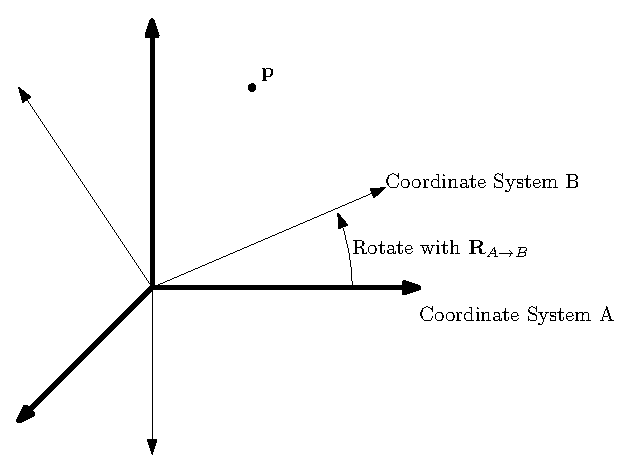
\includegraphics[width=8cm]{Math_transform/coordinateRotate.eps}
\end{figure}




\end{frame}
%%%%%%%%%%%%%%%%%%%%%%%%%%%%%%%%%%%%%%%%%%%%%%%%%%%%%%%%%

%%%%%%%%%%%%%%%%%%%%%%%%%%%%%%%%%%%%%%%%%%%%%%%%%%%%%%%%%
\begin{frame}[fragile]{회전과 이동이 함께 이뤄진 좌표계 변환 (1/2)}

\begin{figure}
    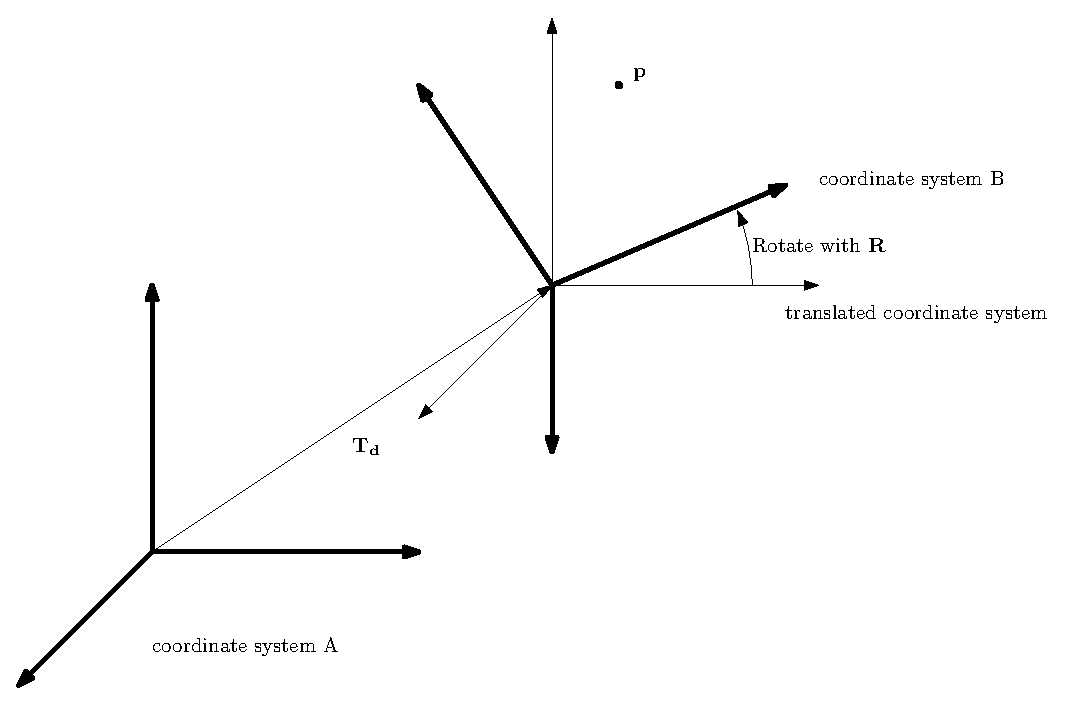
\includegraphics[width=10cm]{Math_transform/coordinateTransform.eps}
\end{figure}


\end{frame}
%%%%%%%%%%%%%%%%%%%%%%%%%%%%%%%%%%%%%%%%%%%%%%%%%%%%%%%%%

%%%%%%%%%%%%%%%%%%%%%%%%%%%%%%%%%%%%%%%%%%%%%%%%%%%%%%%%%
\begin{frame}[fragile]{회전과 이동이 함께 이뤄진 좌표계 변환 (1/2)}

$ 
\mathbf R = \left [ \begin{array}{cc} \mathbf R_{33} & 0 \\ \mathbf O_3^{row}  & 1 \end{array} \right ]
,~~~~$
$ 
\mathbf T_{\mathbf d} = \left [ \begin{array}{cc} \mathbf I_{33} & \mathbf d \\ \mathbf O_3^{row} & 1 \end{array} \right ]
,~~~~$
$ 
\mathbf T_{\mathbf d} \mathbf R = \left [ \begin{array}{cc} \mathbf R_{33} & \mathbf d \\ \mathbf O_3^{row} & 1 \end{array} \right ]
$


\begin{eqnarray}
\mathbf p_A &= 
\left [ \begin{array}{cc} \mathbf R_{33} & \mathbf d \\ \mathbf O_3^{row} & 1 \end{array} \right ]
\mathbf p_B & \nonumber \\
\mathbf p_B &=  
\left [ \begin{array}{cc} \mathbf R_{33}^{\rm T} &  \mathbf R_{33}^{\rm T} \mathbf d \\ \mathbf O_3^{row} & 1 \end{array} \right ]
\mathbf p_A  \nonumber
\end{eqnarray}

\end{frame}
%%%%%%%%%%%%%%%%%%%%%%%%%%%%%%%%%%%%%%%%%%%%%%%%%%%%%%%%%


\end{document}


